%
% Unless otherwise indicated, the copyright in this material is 
% owned by Joerg Evermann. This material is licensed to you under the 
% Creative Commons by-attribution non-commercial license (CC BY-NC 4.0)}
%

\section*{Sources and Further Reading}

The material in this chapter is based on the following sources.

\begin{tcolorbox}[colback=alert]
Molnar, Christoph: \emph{Interpretable Machine Learning} (2023) \\

\url{https://christophm.github.io/interpretable-ml-book/} \\

(CC BY-NC-SA License)
\end{tcolorbox}

Christoph Molnar's book is a very readable and fairly comprehensive introduction to interpretable machine learning or explainable artificial intelligence (XAI). It provides only a few mathematical formulas for illustration and explanation and otherwise relies on intuitive and easy-to-understand descriptions and explanations. It points to and uses software for R and Python, but is not focused on code.

\begin{tcolorbox}[colback=alert]
SciKit-Learn: \url{https://scikit-learn.org/}
\end{tcolorbox}

SciKit-Learn is a comprehensive machine learning framework for Python that also provides some interpretable ML functions. It provides many commonly used as well as advanced functions for classification, regression, and clustering, as well as methods for data preprocessing and model validation and selection.

\begin{tcolorbox}[colback=alert]
PyALE: \url{https://pypi.org/project/PyALE/}
\end{tcolorbox}

PyALE is a Python package to compute Accumulated Local Effects. It is based on an R package with similar functionality and provides ALE plots for numerical and categorical features.

\begin{tcolorbox}[colback=alert]
LIME: \url{https://github.com/marcotcr/lime}
\end{tcolorbox}

LIME is a Python package to compute Local Interpretable Model Explanations (a local model-agnostic method). The package was developed by the authors of the original paper that developed and introduced this method. LIME can be used to explain tabular predictions as well as text- and image-based predictions.

\begin{tcolorbox}[colback=alert]
SHAP: \url{https://shap.readthedocs.io/en/latest/}
\end{tcolorbox}

SHAP is a Python package to compute Shapley Additive Explanations (a local model-agnostic interpretation method). The package was created by the authors of the paper that initially developed the method. SHAP can provide explanations for tabular, text and image predictions. 

%To install these packages and dependencies, use the following command from the bash command line

%\begin{bashcode}
%pip install statsmodels matplotlib scikit-learn PyALE lime shap
%\end{bashcode}

\section{Introduction}

Many machine learning models, in particular non-linear, deep neural network models, are too complex for humans to comprehend or grasp. Such models can have millions or even billions of trainable parameters in complex architectures that may include convolutions, LSTM cells, and other complex elements. These kinds of models are known as ''black box'' models\index{Black-box model}, because their inner workings are essentially inscrutable.

Interpretable machine learning refers to the techniques and models where the processes and results they produce can be understood by human beings. The aim of interpretable machine learning is to ensure human understanding of how the machine learning models work and how they arrive at their results, that is, their decisions or predictions. In other words, it is about \emph{why} a decision or prediction is made, in understandable terms. 

\subsection*{Motivation}

This interpretability is crucial for various aspects from debugging models to compliance with legal standards. Interpretable machine learning is important for a number of reasons:

\begin{itemize}
\item \emph{Curiosity:} Interpretable models satisfy human curiosity about how decisions are made, especially in systems affecting our daily lives. Understanding the decision process can foster deeper insights and innovations.

\item \emph{Human Learning:} By interpreting machine learning models, humans can learn new patterns and knowledge about the data and the phenomena they model, potentially leading to academic advancements and practical applications.

\item \emph{Human Sensemaking of Events and Phenomena:} Interpretability helps users make sense of automated decisions and the events or actions that are consequences of such decisions, ensuring that outcomes are understandable in human terms.

\item \emph{Knowledge Extraction for Scientific Progress:} Interpretable models allow scientists and researchers to extract and verify new knowledge from complex datasets, advancing scientific understanding.

\item \emph{Safety and Compliance Assessment:} Ensuring that machine learning systems operate safely and within regulatory frameworks is easier when these systems are interpretable. Stakeholders can verify compliance through understandable model outputs.

\item \emph{Reliability and Robustness Evaluation:} Interpretable models facilitate the evaluation of system reliability and robustness by making it possible to assess how decisions are made under various conditions.

\item \emph{Identify Knowledge Limits:} Interpretable models help identify the limits of the knowledge embedded in the models, including areas where the model may lack information or where it is unreliable.

\item \emph{Auditability:} Being able to audit machine learning processes transparently helps in maintaining accountability, particularly in sectors like finance and healthcare.

\item \emph{Bias Detection \& Ensuring Fairness:} Interpretability is key in detecting biases in model predictions and ensuring that machine learning applications are fair and do not perpetuate or exacerbate existing inequalities.

\item \emph{Trust and Acceptance:} Users are more likely to trust and accept machine learning solutions that they can understand and feel confident that they are fair and effective.

\item \emph{Debugging \& Failure Analysis:} When a model's decisions can be traced and understood, identifying errors and the reasons for failures becomes feasible, allowing for more effective debugging and correction.

\item \emph{Legal Obligations (''Right to Explanation''):} In many jurisdictions, regulations such as GDPR mandate that decisions made by automated systems be explainable to affected individuals, fulfilling legal obligations.
\end{itemize}

\subsection*{Intrinsic and Post-Hoc Interpretability}

Interpretability\index{Interpretability} in machine learning can be broadly classified into two categories: intrinsic interpretability and post-hoc interpretability. These two types represent different approaches and philosophies in making machine learning models understandable to humans. 

\emph{Intrinsic interpretability}\index{Interpretability!intrinsic} refers to the use of machine learning models that are naturally understandable due to their simple structure and the simplicity of their decision-making process. These models are known as ''white box'' models\index{White-box model} and are designed to be interpretable from the ground up, with the following important characteristics:

\begin{itemize}
\item \emph{Simplicity:} Models such as linear regression, decision trees, or logistic regression are considered intrinsically interpretable because their decisions can be easily traced to their input features and understood without requiring additional tools or techniques.
\item \emph{Transparency:} The model's workings are transparent, meaning that each step of the decision process is visible and comprehensible to users.
\item \emph{Limited Complexity:} These models typically involve fewer parameters and simpler relationships, which aids in direct human comprehension.
\end{itemize}

Post-hoc interpretability\index{Interpretability!post-hoc} involves techniques and methods applied after model training to explain or clarify how a model makes decisions. This is often necessary for complex models like neural networks or ensemble methods that combine multiple classifiers, where intrinsic interpretability is not feasible. Methods such as LIME (Local Interpretable Model-agnostic Explanations), SHAP (SHapley Additive exPlanations), or feature importance metrics are commonly used to provide insights into model decisions. These methods do not depend on the model type; they can be applied to any model type. Post-hoc methods are designed to be used externally to the original black box model, making them versatile in application and providing flexibility in model choice and deployment.

The choice between intrinsic and post-hoc interpretability depends on the balance between the need for prediction accuracy and the requirement for transparency or understandability. While intrinsic interpretability is preferable for clarity and ease of understanding, the simplicity and limited complexity often (but not always) means that these models have lower predictive performance. Post-hoc interpretability provides critical insights into complex models, ensuring that even the most sophisticated algorithms can be scrutinized and understood. However, the understanding is often limited to the output only, rather than the method by which a model generates output. That is, the interpreted model remains a somewhat opaque black-box model.

\subsection*{Local and Global Interpretation}

Interpretation methods are often categorized into local and global methods. Each type provides different insights into the functioning of machine learning models, tailored to specific needs and scenarios.

\emph{Local interpretation methods}\index{Interpretation method!local} focus on explaining individual predictions made by a machine learning model. These methods aim to clarify why a model made a specific classification decision or regression prediction for a particular instance. These methods provide explanations for individual data points, helping to understand the model's behavior at a granular level. Examples include LIME (Local Interpretable Model-agnostic Explanations) and counterfactual explanations, which explain how changes in input features could alter the prediction. Local interpretations are particularly useful in applications like healthcare or finance, where understanding specific decisions is crucial for trust and verification. Typically, local methods focus on the impact of specific feature values.

\emph{Global interpretation methods}\index{Interpretation method!global} seek to explain the overall behavior or logic of a model across all instances. They provide a holistic view of how the model operates in general. These methods explain the model's general decision-making process rather than focusing on individual predictions. Examples include feature importance and partial dependence plots, which show the effect of each feature on the model's predictions across the entire dataset. Global interpretations are beneficial when stakeholders need to validate the model's overall logic and ensure it aligns with domain knowledge and objectives. In contrast to local methods, global methods focus on the impact of features, not the impact of specific feature values.

The choice between local and global interpretation methods depends on the specific needs for transparency in a given application. Local methods are best suited for cases requiring detailed explanations of individual decisions, while global methods are ideal for understanding and validating the overall behavior of a model. 

%\subsection*{Scope of Interpretability}

%Interpretable machine learning involves a variety of concepts that help in understanding how models make decisions.

%\paragraph*{Model and Design Transparency}
%(''Why does the model have the specific architecture?'') 
    %Model and design transparency involves disclosing why a particular model architecture or design was chosen. This includes justifying the use of specific layers in neural networks, the choice of parameters in an algorithm, or the decision to use certain types of data inputs. This transparency helps stakeholders understand the rationale behind model construction, ensuring that the design aligns with the intended applications and performance expectations.

%\paragraph*{Algorithmic Transparency}
%(''How does the algorithm create the trained model?'') 
    %Algorithmic transparency refers to the clarity and openness about how an algorithm operates to convert input data into a trained model. This involves explaining the learning process, the optimization techniques used, and how data is transformed throughout the model training phase. Understanding these aspects is crucial for assessing the model's reliability and for debugging or improving model performance.

%\paragraph*{Global, Holistic Model Interpretability}
%(''How does the trained model make predictions?'') 
    %This concept focuses on understanding the model's overall decision-making process across all possible inputs. It involves explaining how the model integrates and weighs different features to make predictions. Techniques such as feature importance metrics and model summaries help in conveying a broad understanding of how the model functions in general.

%\paragraph*{Global, Modular Model Interpretability} (''How do parts of the model affect predictions?'') 
    %This aspect of interpretability looks at how individual components or modules of a model contribute to the overall predictions. It is particularly relevant in complex models where different parts of the model have distinct roles, such as different layers in deep learning networks or sub-models in ensemble methods.

%\paragraph*{Local Interpretability for a Single Prediction} (''Why did the model make this prediction for this instance?'') 
    %Local interpretability at the individual prediction level involves explaining why the model arrived at a particular decision for a specific instance. Techniques like LIME or SHAP are used to provide insights into which features were most influential for that specific decision, helping users and stakeholders understand the rationale behind individual outputs.

%\paragraph*{Local Interpretability for a Group of Predictions} (''Why did the model make these predictions for these instances?'') 
    %This involves explaining the model's behavior across a group of similar instances or under similar conditions. It helps in understanding model consistency and behavior patterns for specific subsets of data, which is useful for identifying model strengths and weaknesses in handling different types of data situations.

%These interpretability concepts ensure that models are not only effective in their tasks but also align with ethical standards and are accountable in their operations. Providing clarity at various levels -- from the overall model down to individual predictions -- enhances the usability and acceptance of machine learning systems.

\section{Intrinsically Interpretable Models}

Intrinsically interpretable machine learning models often leverage characteristics such as linearity, monotonicity, and interactions to ensure that their workings are transparent and understandable.

\emph{Linearity} in machine learning models means that the output is a linear combination of the input features. Models like linear regression are classic examples where each predictor has a constant effect on the outcome. Linear models are straightforward, making them easy to understand and explain. The impact of each feature on the prediction is clear and quantifiable. The effects of changes in input features are predictable, aiding in scenario analysis and planning.

\emph{Monotonicity} in a model ensures that the relationship between any given input and the output is either always non-decreasing or always non-increasing. Linear regression models and decision trees that split based on a single feature at a time can exhibit this property. Monotonic models are consistent in their behavior, enhancing trust as increases (or decreases) in input variables lead to predictable changes in outputs. These models are easier to validate against domain knowledge, where certain inputs are expected to have a direct and consistent influence on the output.

\emph{Interactions} in machine learning refer to the scenario where the effect of one feature on the response variable depends on the value of another feature. By modeling the interdependencies between features, interaction-enabled models can often achieve higher predictive accuracy while still maintaining a degree of interpretability. Many phenomena involve interdependent factors; accurately modeling these interactions can make the model outputs more applicable and relevant in real-world scenarios.

Linearity, monotonicity, and interactions each play crucial roles in ensuring that intrinsically interpretable machine learning models are both effective and transparent. While linearity and monotonicity contribute to simplicity and predictability, interactions allow for a nuanced understanding of complex dynamics within the data. Table~\ref{tab:intrinsicmodels} shows a list of intrinsically interpretable models. This section examines the emphasized entries in the table, linear regression and decision trees, while others, such as logistic regression, naive Bayes, and k-NN, have been presented and discussed in previous sections.

\begin{table}
\centering
\renewcommand{\arraystretch}{1.1}

\begin{tabular}{lccc} \hline
Algorithm & Linear & Monotone & Interaction \\ \hline
\textbf{Linear regression} & Yes & Yes & No  \\ 
Logistic regression & No & Yes & No  \\
\textbf{Decision trees} & No & Some & Yes  \\
RuleFit & Yes & No & Yes  \\
Naive Bayes & No & Yes & No \\
k-NN & No & No & No  \\ \hline
\end{tabular} \\
\vspace{.5\baselineskip}
\scriptsize Source: \url{https://christophm.github.io/interpretable-ml-book/simple.html}\normalsize

\caption{Intrinsically Interpretable Models}
\label{tab:intrinsicmodels}
\end{table}

\subsection{Linear Regression}

Linear regression is one of the simplest prediction methods available and is intrinsically interpretable\index{Linear regression}. Consider the following example linear regression model for predicting bicycle rental count (variable \texttt{cnt}) from the season (\texttt{season}) and the temperature (\texttt{cnt}) (using R).

\begin{Rcode}
# Load the bike rental data set
d <- read.csv('https://evermann.ca/busi4720/bike.csv')

# Perform the regression and summarize results
summary(lm(cnt~season+temp, data=d))
\end{Rcode}

The abbreviated output below is easy to interpret and demonstrates linearity and  monotonicity. For example, the coefficient for temperature of $132.79$ means that, all other variables remaining the same (''ceteris paribus''), a change of one degree of temperature will change the predicted bicycle rental count by $132.79$, no matter what the original temperature is (linearity) and always in the same direction as the temperature change (monotonicity). 

The coefficients for the categorical season variable are also easy to interpret. They represent the predicted change in bicycle rental count from the reference category (in this case, FALL), assuming all other variables remain the same (''ceteris paribus''). For example, the prediction for the winter is $1342.87$ lower than for the fall.

The intercept is easy to interpret as that prediction when all other variables are $0$, or the reference category for categorical variables. In this example, for a temperature of 0 degrees and in the fall season, the model predicts a rental count of $3151.02$.

\begin{textcode}
Coefficients:
             Estimate Std. Error t value Pr(>|t|)    
(Intercept)   3151.02     169.35  18.606  < 2e-16 ***
seasonSPRING  -494.15     163.28  -3.026  0.00256 ** 
seasonSUMMER  -852.68     209.82  -4.064 5.35e-05 ***
seasonWINTER -1342.87     164.59  -8.159 1.49e-15 ***
temp           132.79      11.02  12.046  < 2e-16 ***
---
Residual standard error: 1433 on 726 degrees of freedom
Multiple R-squared: 0.4558, Adjusted R-squared: 0.4528 
\end{textcode}

The $R^2$ is an easily understood metric to assess the quality of the model. It explains the proportion of variance in the target variable that is explained by the predictors. A good model has an $R^2$ close to 1, while an $R^2$ close to 0 indicates a poor model. 

Finally, the \emph{relative feature importance} is given by the $t=\frac{\hat{\beta}}{SE(\hat{\beta})}$ value. Because it divides the coefficient estimate by its standard error, the t-value is scale invariant and can be used to compare the importance of features on different scales. In the above example, it is clear that temperature is the most important features\index{Feature importance by t-test}.

In summary, it is easy to understand which features are most or least important in making a prediction and how features interact or do not interact (consider what ''ceteris paribus'' implies for interactions). 

Linear regression also has high local interpretability; predictions for individual observations are also easy to understand. For example, to predict the bicycle rental count in summer when the temperature is 20 degrees, one uses the following regression equation, with parameter values from the output above:

\begin{align*}
\hat{c} = 3151.02 - 852.68 + 20 \times 132.79 = 4954.14
\end{align*}

Finally, the ordinary least squares algorithm that is used to compute the model parameters is simple and well-understood and is proven to produce optimal parameter values. This means that linear regression has high \emph{algorithmic transparency}\index{Algorithmic transparency}. In other words, it is clear what the optimization objective is, and how it is achieved. 

To further improve the interpretability of linear regression models, one may try to reduce the number of features or input dimensions, using methods such as:

\begin{itemize}
   \item \emph{Manual feature selection}: The analyst may successively omit less important features, or may include features based on the strength of their correlation with the target variable. 
   \item \emph{Automatic feature selection}: While an exhaustive search of all possible feature combinations is typically not feasible, automated heuristics are able to arrive at a reasonably good subset of features that still provides good prediction capability with a small number of features.
   \item \emph{Regression with PCA components}: PCA produces linear combinations of varaibles with maximal variance. Retaining a few of such components instead of the full set of features may make the model more interpretable. However, the components themselves must also be interpreted, based on their loadings or correlations with the original features. 
   \item \emph{Penalized regression}: The LASSO is a penalized regression that automatically removes features (sets their coefficient to $0$) as a function of the penalty parameter $\lambda$.
\end{itemize} 

In general, the analyst must consider the bias and variance implications of these dimensionality reduction methods: Simpler models will generally have a higher bias and lower variance than more complex models. 

\subsection{Decision Trees}

\emph{Decision trees}\index{Decision tree} are another relatively simple and easy to understand predictive machine learning technique. Decision trees can be used both for regression (''regression trees'') and for classification (''classification trees''). Decision trees are a popular choice in interpretable machine learning due to their strengths:

\begin{itemize}
\item \emph{Algorithmic Transparency:} The procedure to construct a decision tree and the optimization criteria are easy to understand and verify. The optimization criterion to derive the decision rules is simple and intuitive. 
\item \emph{Simplicity:} The structure of a decision tree is simple and intuitive, which allows non-experts to understand the model's reasoning easily. This simplicity also facilitates easier communication about the model's decision-making process.
\item \emph{Visualization:} Decision trees offer a clear visualization of how decisions are made, with each node representing a decision rule and each path a decision process. This makes them highly interpretable and easy to follow.
\item \emph{No Need for Feature Scaling:} Unlike some other machine learning models, decision trees do not require input features to be scaled or normalized. This avoids potential distortions in interpretation due to preprocessing.
\item \emph{Handling of Non-linear Relationships:} Decision trees can handle complex, non-linear relationships between features without needing any transformation of data, capturing interactions between the variables naturally.
\item \emph{Capability to Handle Both Numerical and Categorical Data:} Trees can process datasets that have a mix of numerical and categorical variables without the need for extensive preprocessing.
\end{itemize}

However, decision trees have a number of weaknesses that may limit their usefulness or applicability to certain problems. 

\begin{itemize}
\item \emph{Overfitting:} Decision trees are prone to overfitting, especially for very deep trees. Without aggressive tree ''pruning'', they can create overly complex trees that do not generalize well.

\item \emph{Instability:} Small changes in the data can result in a completely different tree being generated. In other words, they have high variance.

\item \emph{Bias Towards Certain Structures:} Decision trees tend to favor splits on features having a larger number of levels. This can bias the model's decision-making process, especially if the feature's relevance is artificially inflated by its structure.

\item \emph{Greedy Nature:} Standard algorithms for decision tree construction, such as CART (Classification and Regression Trees, discussed below), are greedy because they make the best split at a given node without considering future impacts. This might lead to suboptimal trees.

\item \emph{Piecewise Constant Predictions:} Decision trees make piecewise constant decisions, that is, they predict the same values or classes within small regions of the feature space. This means that the predictions within these spaces have zero variance, which may be problematic for subsequent analytics. 
\end{itemize}


\begin{figure}
\centering
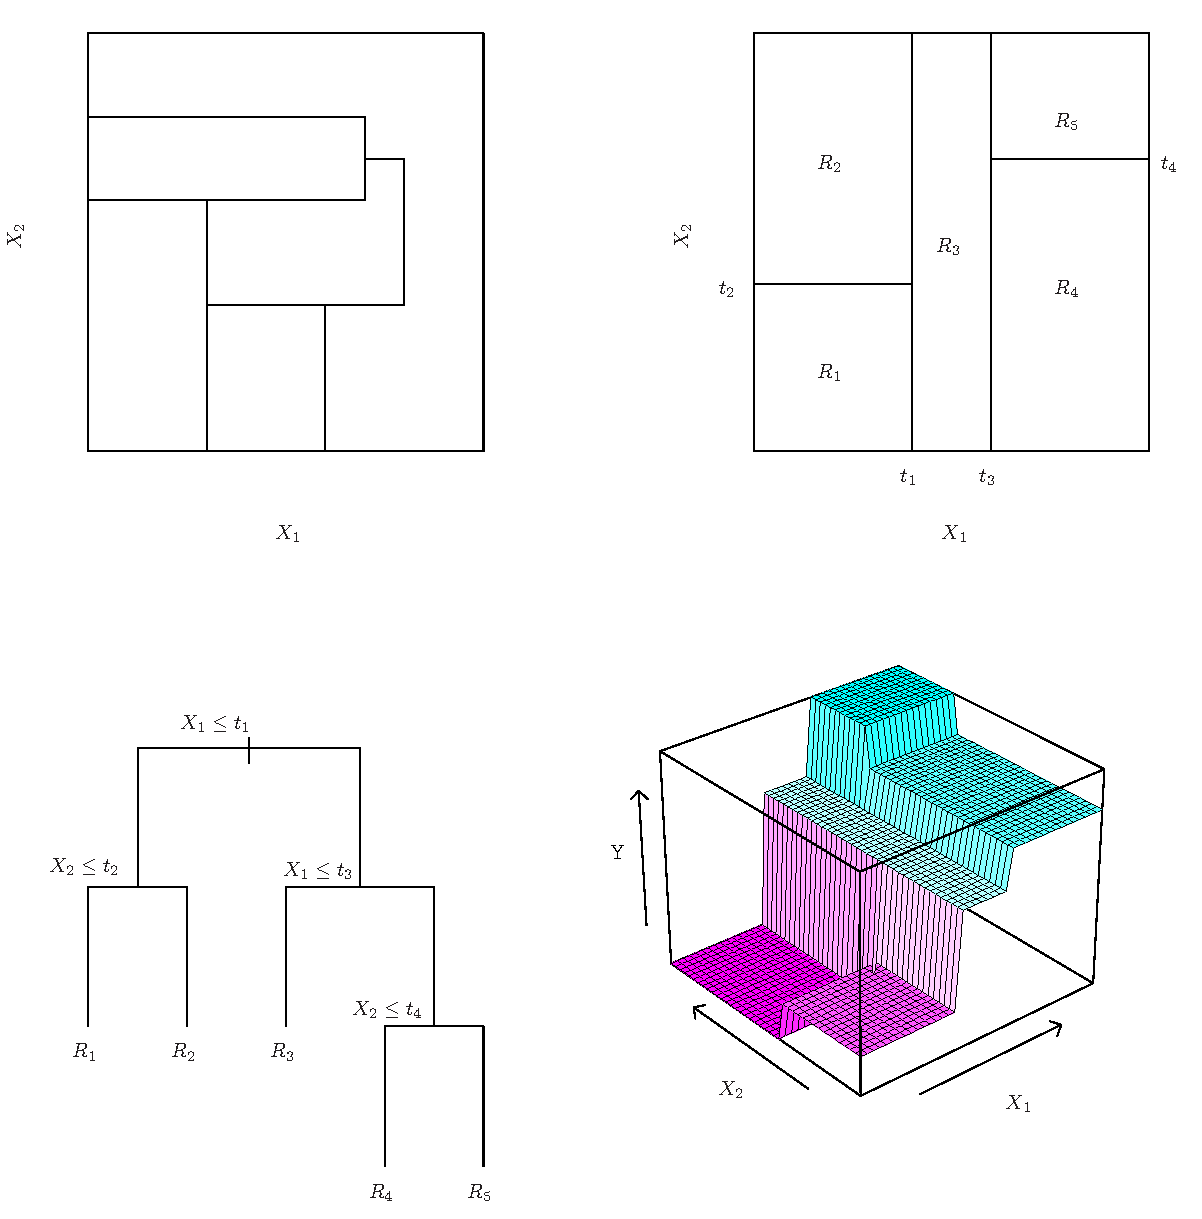
\includegraphics[width=.75\textwidth]{../class11/Figures_Chapters_7-13/Chapter8/8_3.pdf} \\

\scriptsize Source: ISLR2 Figure 8.3
\caption{Decision tree for two numerical features}
\label{fig:decisiontree}
\end{figure}

Figure~\ref{fig:decisiontree} shows the intuition behind binary decision trees. The top left panel in the figure shows a feature space spanned by two numerical features, $x_1$ and $x_2$. The space is subdivided into regions where predictions on the target variable are similar. Unfortunately, an optimal sub-dividing of the feature space is difficult to achieve when the regions are irregularly shaped. Instead, binary decision trees are created by making a binary split of the feature space along one feature/dimension, yielding two smaller regions. Each region may then be split again, recursively, until a stopping criterion is reached. 

Consider the top right panel in Figure~\ref{fig:decisiontree} as an example. Here, the feature space is first split on feature $x_1$ at value $t_1$ creating two rectangular regions, one to the left of $t_1$ where $x_1 \leq t_1$ and the other to the right where $x_1 > t_1$. The left region is then split on feature $x_2$ at value $t_2$ creating the regions labelled $R_1$ where $x_1 \leq t_1 \wedge x_2 \leq t_2$ and $R_2$ where $x_1 \leq t_1 \wedge x_2 > t_2$. These two regions are not split any further, and are called the ''leafs'' or ''leaf nodes'' of the tree. The region to the right of $t_1$, that is the region where $x_1 > t_1$, is split again on feature $x_1$ at value $t_3$, yielding the region $R_3$ where $x_1 > t_1 \wedge x_1 \leq t_3$ and the region where $x_1 > t_1 \wedge x_1 > t_3$. The latter region is split on feature $x_2$ at value $t_4$, yielding regions $R_4$ and $R_5$. 

The bottom left panel in Figure~\ref{fig:decisiontree} shows how these split or divisions of the feature space form a (upside down) decision tree with root, decision nodes, and the resulting leaf nodes. The bottom right panel in Figure~\ref{fig:decisiontree} shows what a prediction of a target variable (here, a numerical target), might look like. For a regression tree\index{Regression tree}, the predicted value for each region is simply the average of the observed target values in each region, leading to the flat plateaus shown in the bottom right panel, that is, piece-wise constant predictions for small regions of the feature space. For a classfication tree\index{Classification tree}, the predicted class for a leaf node is simply the majority class of observations in each region. 

For binary decision trees, the choice on which feature to split on next and which specific feature value to split on is decided as follows:
\begin{enumerate}
   \item For every feature $j$ and potential split feature value $s$ define regions
   \begin{align*}
   R_1(j,s) = \{X | X_j < s\} \quad &\text{and} \quad R_2(j, s) = \{X | X_j \geq s\}
   \end{align*}
   This is simple for binary feature but requires dichotomization or discretization (for example, using equal interval bins or equal frequency bins) for numerical features and can potentially result in a large number of possible split points $s$.
   \item Use one of the following criteria to choose $j$ and $s$:
   \begin{itemize}
      \item \emph{Minimize the total variance of the two regions (regression trees)}:
      \begin{align*}
       \sum_{i: x_i \in R_1(j,s)} (y_i - \bar{y}_{R_1})^2 &+ \sum_{i: x_i \in R_2(j,s)} (y_i - \bar{y}_{R_2})^2
       \end{align*}
       The decision tree algorithm will calculate the total variance of both groups resulting from each potential split and then choose the split that will yield the lowest variance.
      \item \emph{Maximize information gain (classification trees)}:
      Recall that the entropy is defined as 
	  \begin{align*}
	   H(Y) = - \sum_{y \in Y} p(y) \log p(y)
	   \end{align*}
       where $p(y)$ represents the proportion of each class $y$ in a child node. The information gain\index{Information gain (in decision trees)} obtained by splitting on a feature $j$ at feature value $s$ and forming regions $R_1$ and $R_2$ is then defined as:
	   \begin{align*}
	   IG(Y, a) = H(Y) - p(R_1) H(Y | R_1) - p( R_2) H(Y | R_2) 
	   \end{align*}
       where $p(R_1)$ is the probability of an observation being in region $R_1$, that is, the proportion of observations in region $R_1$, and $H(Y | R_1)$ is the conditional entropy, that is, the entropy of those observations in region $R_1$ (analogous for $R_2$. 
       
       Intuitively, the entropy $H$ expresses the uncertainty in the distribution of $Y$. Knowing or assuming a value (or range of values) for some feature $j$ should decrease the uncertainty, that is, lead to a gain in information. The decision tree algorithm will calculate the information gain resulting from each split and will choose the split with the highest gain.
   \item \emph{Minimize Gini index (classification trees)}:
   The Gini impurity\index{Gini impurity index} of a dataset is defined as:
\begin{align*}
Gini = 1 - \sum_{i=1}^k p(y)^2
\end{align*}
where $p(y)$ is the probability of an observation being classified to a particular class $y$. The Gini impurity index represents the probability of an observation being misclassified if it were randomly assigned a label according to the distribution of classes in the data at that node. A Gini impurity of 0 indicates that all cases in the node fall into a single category, i.e., the node is completely pure. The decision tree algorithm will calculate the Gini impurity for each subgroup that would result from a split and will choose the split that results in the lowest weighted sum of the group impurities.
\end{itemize}
\end{enumerate}

The above process is recursively repeated for each region, resulting in a tree that is growing new leaf nodes and gaining depth. Without any stopping, the tree will grow, that is, nodes will be split, until every leaf node contains only a single observations. It is clear that such a fully-grown tree is overfitted to the training data set, and not easily interpretable. 

In practice, to prevent overfitting and ensure the tree remains interpretable, the splitting process is stopped using one many options for \emph{stopping criteria}:

\begin{itemize}
  \item \emph{Maximum tree depth}: The splitting of the feature space stops when a specified tree depth is reached. All branches of the tree have the same depth/length. 
  \item \emph{Maximum leaf node count}: Splitting of the feature space stops when a certain number of leaf nodes have been created. Not all branches of the tree need to have the same length/depth. This limits the number of decisions in the decision tree and the number of unique predicted values for regression trees.
  \item \emph{Minimum Leaf node sample size}: Leaf nodes must have a minimum number of observations. This makes the predictions for each feature space region more representative as they are based on a minimum sample size.
  \item \emph{Maximum leaf node variance}: Splitting continues until the variance of observations in a regression tree regions is below a certain threshold. 
  \item \emph{Minimum leaf node purity}: Regions are split while they contain a mixture of target observations; splitting stops only when a node contains a certain proportion of a majority class for classification trees or when the entropy is below a certain threshold. This criterion prevents unnecessary splitting which may result in two sub-regions yielding the same predicted class. 
  \item \emph{Minimum change in node impurity or information gain}: Regions are split while the improvement in purity or reduction of entropy are above a certain threshold. This criterion prevents unnecessary splits that do not significantly improve the predictive power of the model. 
\end{itemize}

To illustrate decision trees, consider the following Python example, using the \\ \texttt{DecisionTreeRegressor} class from the SciKit-Learn package. The example uses the same data set as the linear regression example above and constructs a regression tree to predict the count of bicycle rentals from the temperature and humidity, two numerical variables. 

The example fits an unpruned tree, that is, there is no stopping criterion and the tree will have as many leaf nodes as there are observations. Consequently, there will be no prediction error for the training data and the tree is very much overfitted.

\begin{samepage}
\begin{pythoncode}
import matplotlib.pyplot as plt
import pandas as pd
# Prepare data:
d=pd.read_csv('https://evermann.ca/busi4720/bike.csv')
x=d[['temp', 'hum']]
y=d['cnt']
#Fit unpruned tree:
from sklearn.tree import DecisionTreeRegressor
regr = DecisionTreeRegressor()
regr.fit(x, y)
# Print the MSE:
from sklearn.metrics import mean_squared_error
mean_squared_error(regr.predict(x), y)
\end{pythoncode}
\end{samepage}

Early stopping can prevent overfitting and maintain interpretability. The following three examples show how to use the tree depth criterion, the leaf node sample size criterion and the leaf node count criterion for stopping the tree construction. Each of those trees will have a non-zero training error.

\begin{samepage}
\begin{pythoncode}
regr = DecisionTreeRegressor(max_depth=3)
regr.fit(x, y)
regr = DecisionTreeRegressor(min_samples_leaf=10)
regr.fit(x, y)
regr = DecisionTreeRegressor(max_leaf_nodes=8)
regr.fit(x, y)
\end{pythoncode}
\end{samepage}

To demonstrate the interpretability of a decision tree, it is useful to print the tree and to visualize or plot the tree. 

\begin{samepage}
\begin{pythoncode}
import sklearn
# Print the tree:
print (sklearn.tree.export_text(regr, feature_names=x.columns))
# Plot the tree:
sklearn.tree.plot_tree(regr, max_depth=2, feature_names=x.columns, 
    filled=True, fontsize=6)
plt.show()
\end{pythoncode}
\end{samepage}

Printing the fitted tree will show the decision nodes and the predicted value of each leaf node, which is simply the mean value of the observations for that leaf node. The output from the Python code above is shown below. Plotting the tree results in the visualization shown in Figure~\ref{fig:regtree}. It is clear that decision trees have good local interpretability, that is, for a given observation, it is easy to see how the tree model arrives at its predictions. However, global interpretability is lacking. For example, it is unclear whether temperature or humdity is the more important predictor in this example. One could count the number of splits that are based on a particular variable to gain an idea of its importance, but this is a pretty rough approximation. 

\begin{figure}
\centering

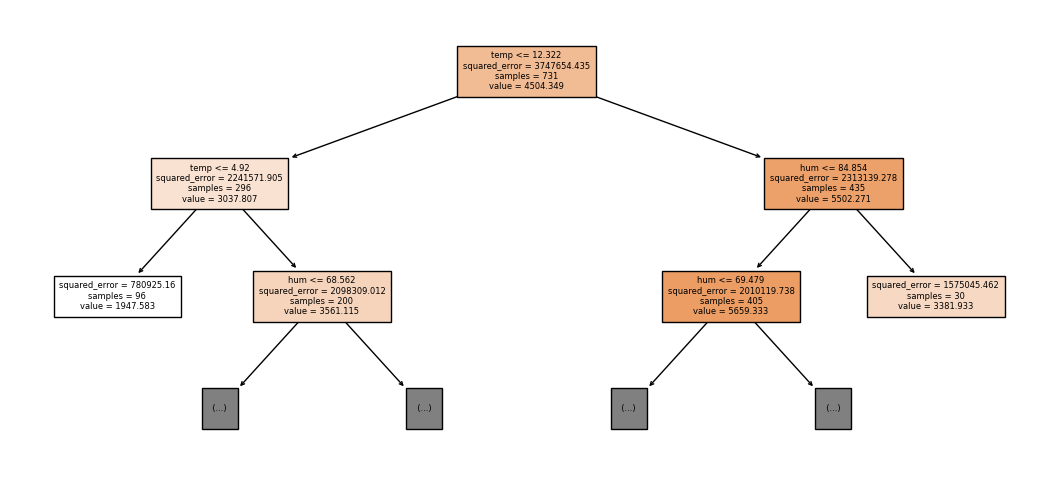
\includegraphics[width=.8\textwidth]{reg_tree.png}
\caption{Regression tree example}
\label{fig:regtree}
\end{figure}

\begin{samepage}
\begin{textcode}
|--- temp <= 12.32
|   |--- temp <= 4.92
|   |   |--- value: [1947.58]
|   |--- temp >  4.92
|   |   |--- hum <= 68.56
|   |   |   |--- value: [3885.62]
|   |   |--- hum >  68.56
|   |   |   |--- value: [2916.96]
|--- temp >  12.32
|   |--- hum <= 84.85
|   |   |--- hum <= 69.48
|   |   |   |--- temp <= 17.40
|   |   |   |   |--- value: [5355.81]
|   |   |   |--- temp >  17.40
|   |   |   |   |--- temp <= 23.51
|   |   |   |   |   |--- value: [6698.34]
|   |   |   |   |--- temp >  23.51
|   |   |   |   |   |--- value: [5716.78]
|   |   |--- hum >  69.48
|   |   |   |--- value: [5183.22]
|   |--- hum >  84.85
|   |   |--- value: [3381.93]
\end{textcode}
\end{samepage}

Finally, to show the piecewise constant predictions across small regions of the feature space, consider the scatter plot of predicted values in Figure~\ref{fig:treescatter}, created using the following Python code block. The plot shows the actual target on the horizontal axis and the predicted target on the vertical axis. Predictions for different actual target values are the same. From the graph, it is evident that the tree has eight leaf nodes corresponding to those in the printed output, that is, the tree is able to predict 8 different values. 

\begin{samepage}
\begin{pythoncode}
# Plot fitted versus true values:
import plotly.express as px
px.scatter(pd.DataFrame([y, regr.predict(x)], \
    index=['y', 'yhat']).transpose(),x='y', y='yhat').show()
\end{pythoncode}
\end{samepage}

\begin{figure}
\centering
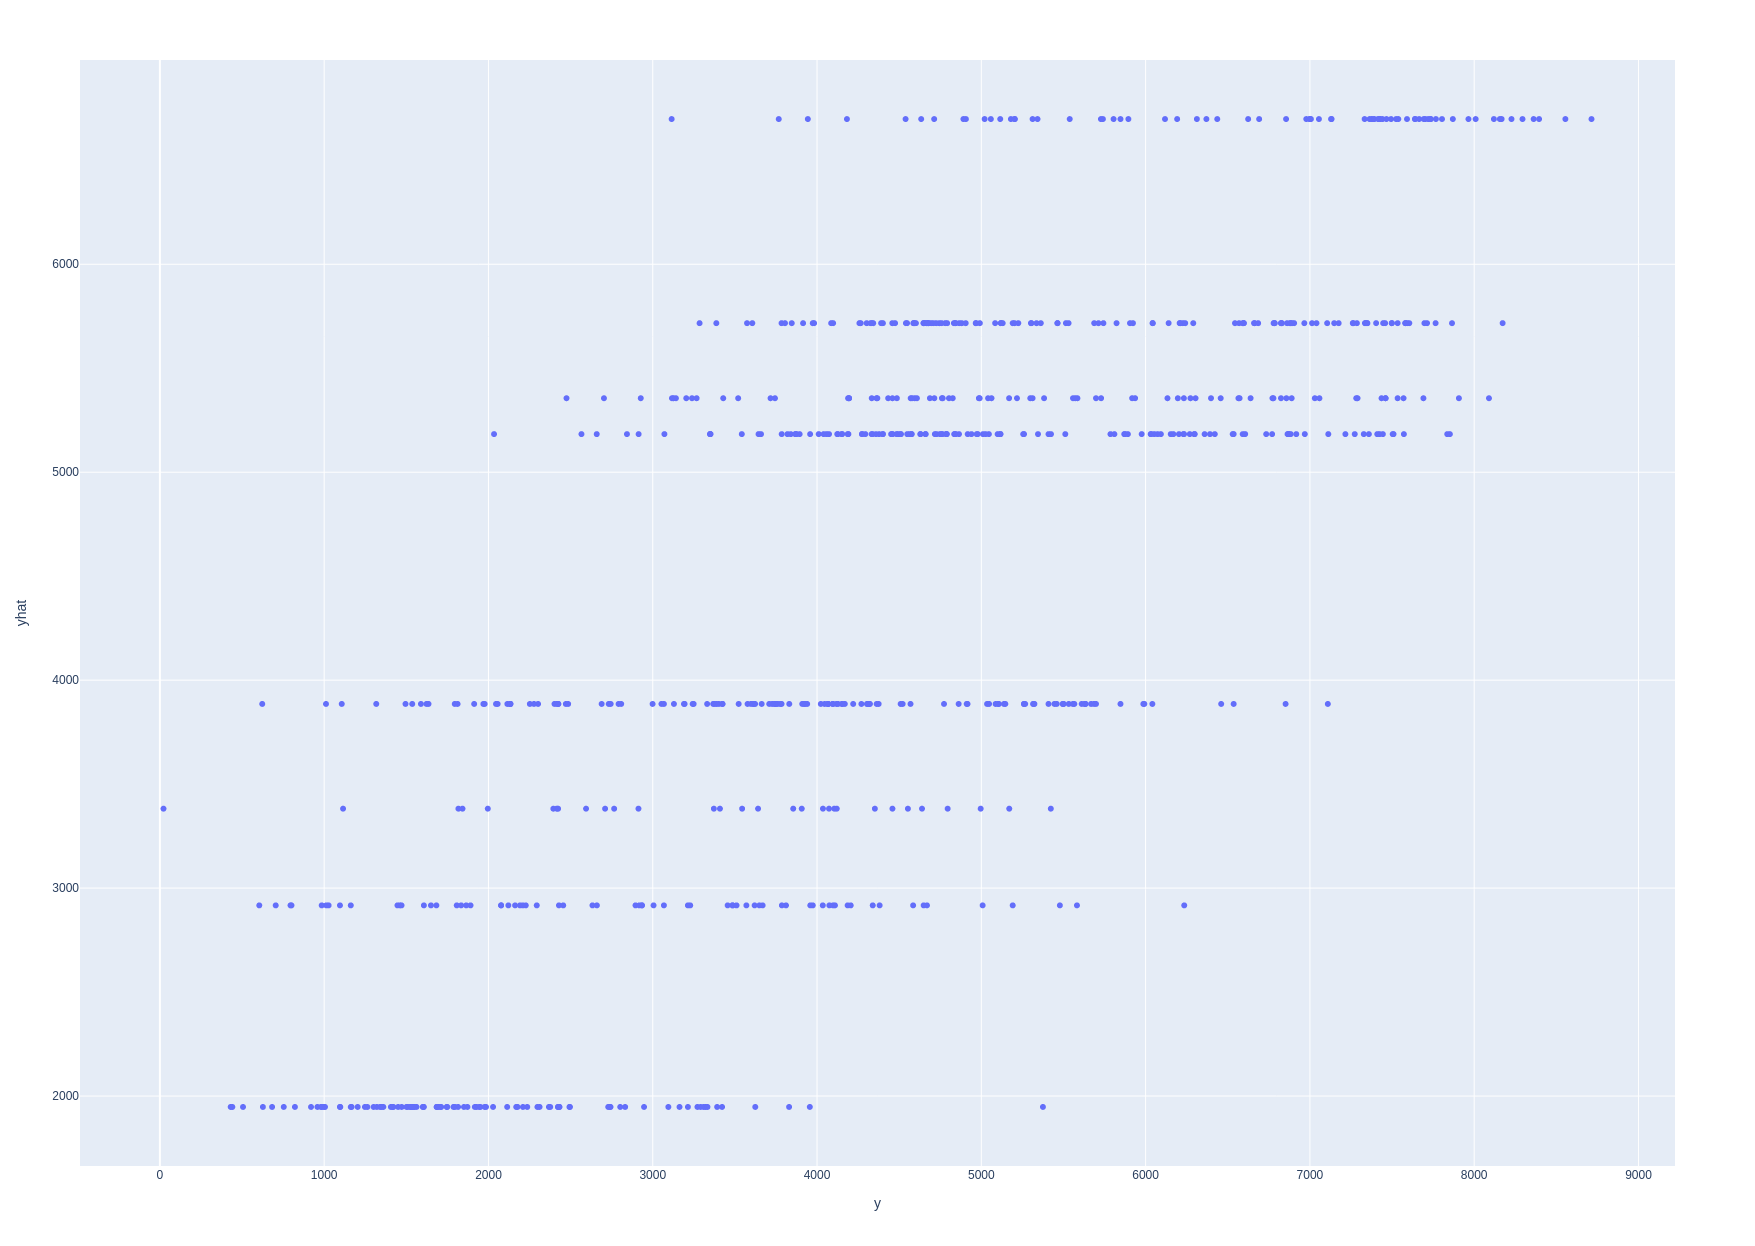
\includegraphics[width=\textwidth]{tree_fitted_true2.png}
\caption{Predictions of a regression tree}
\label{fig:treescatter}
\end{figure}

\begin{tcolorbox}[colback=code]
\subsubsection*{Hands-On Exercise} 

\begin{enumerate}
\item Fit regression trees to the bike dataset in the above examples. Calculate the MSE, print the decision rules, and plot predicted versus true values as you vary the following stopping rule criteria:
\begin{itemize}
   \item \texttt{max\_depth}: choose values 1, 3, 5, 7
   \item \texttt{min\_samples\_leaf}: choose values 1, 5, 10, 20
   \item \texttt{max\_leaf\_nodes}: choose values 2, 8, 16, 32
\end{itemize}
How does the training MSE change? What can you observe from the plots of predicted versus true values?

\item Split the data set into a training and test sample. Repeat exercise (1) but now evaluate the test MSE. What is the optimal stopping criterion?
\end{enumerate}
\end{tcolorbox}

\section{Global Model-Agnostic Methods}

Global model-agnostic interpretation methods\index{Global model-agnostic interpretation method} focus on the understanding the overall impact of features in determining the prediction. They are applicable to different models and focus only on the input features and predictions, while ignoring the specific model or algorithm. This section presents a few of the many methods that have been proposed and developed in recent years. 

\subsection{Partial Dependence Plots (PDP)}

Partial Dependence Plots (PDPs)\index{Partial dependence plot}\index{PDP|see{Partial dependence plot}} provide insights into the relationship between a feature and the predicted outcome, averaged over the distribution of values of the other features in the dataset. By isolating the effect of one or two features, PDPs can show how changes in these features impact the predicted outcome, irrespective of the values of other variables, offering a global view of the model's mechanics.

Formally, a PDP shows the marginal effect of one or a few features $X_S$ on the predicted output, marginalized over all other (''complement'') features $X_C$. Recall that marginalization is the summing, or integration for continuous features, weighted by probabilities:

\begin{align}
\hat{f}_S(X_S) &= \mathbbm{E}_{X_C} \left[ \hat{f}(X_S, X_C)) \right] \nonumber \\
&= \int \hat{f}(X_S, X_C) p(X_C) dX_c \nonumber 
\intertext{When estimated from sample data, this becomes:}
\hat{f}_S(X_S) &= \frac{1}{n}\sum_{i=1}^n \hat{f}(X_S, X_C^{(i)}) \label{eq:pdp}
\end{align}

where the sum in Equation~\ref{eq:pdp} is over all observations and $X_C^(i)$ are the complement feature values of the i-th observations. The integrals or sums are computed for all possible values of $X_S$ to generate the PDP curves. Essentially, the PDP shows shows how the \emph{average} prediction changes when the focal predictor $X_S$ is changed. \emph{Importantly, PDPs assume feature independence}.

Consider the following example in Python. For ease of illustration, the example explains a decision tree model, which is of course intrinsically interpretable already. The example uses the bike rental data set from above and first fits a regression tree.

\begin{samepage}
\begin{pythoncode}
# Read the data set and identify features and target
import pandas as pd
d=pd.read_csv('https://evermann.ca/busi4720/bike.csv')
x=d[['temp', 'hum']]
y=d[['cnt']]
# Fit a regression tree:
from sklearn.tree import DecisionTreeRegressor
regr = DecisionTreeRegressor(max_depth=5).fit(x, y)
\end{pythoncode}
\end{samepage}

Once the model is fitted, the \texttt{PartialDependenceDisplay} class in the Scikit-Learn package can be used to generate a PDP. The \texttt{features} argument indicates which features to use for the PDP. This example Python code below shows individual PDPs for the first and second feature and a joint feature PDP for those two features as well. The \texttt{grid\_resolution} argument controls the discretization of continuous features into equal intervals for summing/marginalization. Figure~\ref{fig:pdp} shows the resulting PDPs. For example, the left panel shows how the prediction varies when the temperature value changes. For each value of temperature, the sum in Equation~\ref{eq:pdp} is computed to calculate the average prediction for that temperature value.

\begin{samepage}
\begin{pythoncode}
import matplotlib.pyplot as plt
from sklearn.inspection import PartialDependenceDisplay
PartialDependenceDisplay.from_estimator(
    estimator = regr, 
    X = x, features = [0, 1, (0,1)], grid_resolution = 20)
plt.show()
\end{pythoncode}
\end{samepage}

\begin{figure}
\centering
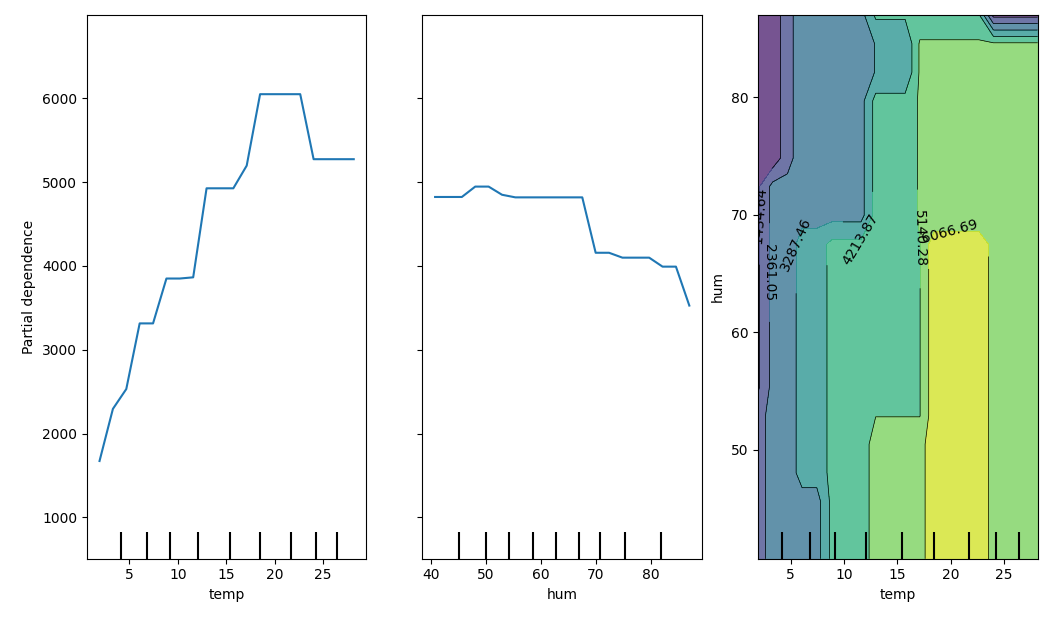
\includegraphics[width=.75\textwidth]{pdp_dtr.png}
\caption{Example PDP for a regression tree}
\label{fig:pdp}
\end{figure}

\emph{Importantly, the PDP removes the ''ceteris paribus'' assumption that linear regression models make. Instead of assuming that all other values remain unchanged, the PDP marginalizes (''averages'') over the values of other features.}

\subsection{Individual Conditional Expectation (ICE) Curves}

Individual Conditional Expectation (ICE)\index{Individual conditional expectation curve}\index{ICE curve|see{Individual conditional expectation curve}} curves extend the idea of PDPs by disaggregating the effects for individual observations. Instead of an average effect over all observations or feature values, an ICE plot displays one curve per instance in the dataset, showing how predictions change for that instance if the feature of interest is varied. This essentially means that no summation in Equation~\ref{eq:pdp} takes place; the ICE curves are simply the individual summands of that sum. Thus, averaging all ICE curves yields the PDP curve. This allows identification of outlier cases or heterogeneous data. 

ICE plots can created in Python using the same way as PDPs. The result of the following Python code block is shown in Figure~\ref{fig:ice}. While the bike rental data set in this example has 731 observations, the ICE plot in Figure~\ref{fig:ice} shows fewer lines because of the piece-wise constant predictions (the fitted tree has 31 leaf nodes), that is, the predictions for multiple observations are identical and the lines are overlaid on top of each other in the ICE plot. From Figure~\ref{fig:ice} it is clear that not all observations follow the same, average pattern and that there is significant heterogeneity in the data set.

\begin{pythoncode}
PartialDependenceDisplay.from_estimator(regr, x, [0, 1], kind='both')
\end{pythoncode}

\begin{figure}
\centering

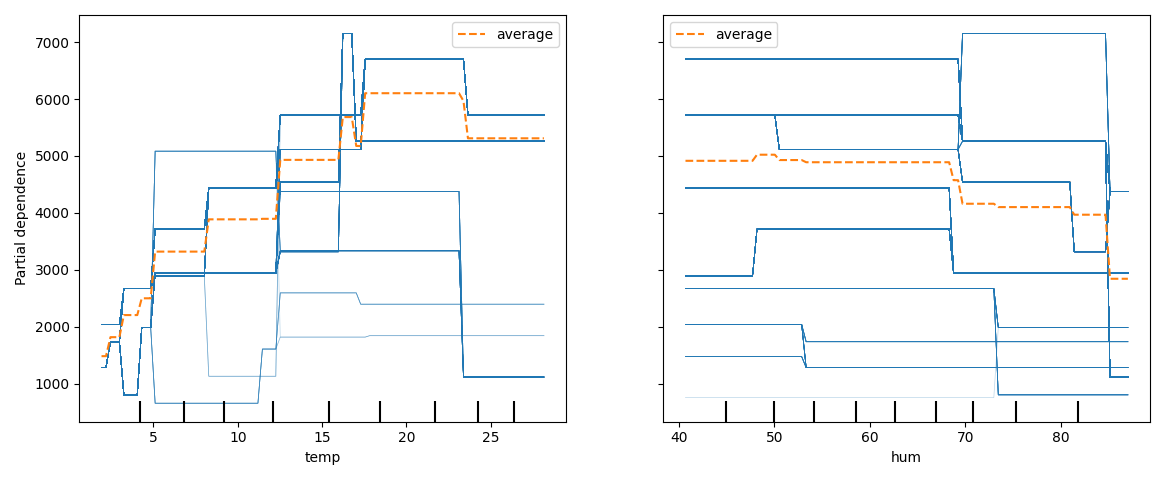
\includegraphics[width=.75\textwidth]{ice_pdp_reg.png}
\caption{Example ICE plot for a regression tree}
\label{fig:ice}
\end{figure}


\subsection{Accumulated Local Effects (ALE) Plot}

Accumulated Local Effects (ALE) plots\index{Accumulated local effect plot}\index{ALE plot|see{Accumulated local effect plot}} address some limitations of PDPs by focusing on local rather than global average effects of features. ALE plots calculate the contributions of features to predictions by accumulating localized average partial effects, helping to avoid misleading interpretations in the presence of correlated features. 

Specifically, ALE plots do not construct unrealistic feature combinations as they average over the complement feature values. For example, the temperature and humidity features are mildly correlated in the running example, and not all combinations are realistic. Instead, effects are computed for a grid of intervals, that is, a ''local window'', instead of the entire domain of a features, as in PDPDs.

Formally, the ALE is defined as:

\begin{align}
\hat{\tilde{f}}_{j, ALE}(X) &= \sum_{k=1}^{k_j(x)} \frac{1}{n_j(k)} \sum_{i:x_j^{(i)} \in N_j(k)} \left[\hat{f}(z_{k, j}, x^{(i)}_j) - \hat{f} (z_{k-1, j},x^{(i)}_j) \right] \label{eq:ale}
\end{align}

The range of values for feature $j$ is divided into $k$ equal size intervals. $N_j(k)$ is the $k$-th such local neighbourhood for a feature $j$ with $Z_{k,j}$ being the lower boundary of that interval. The summands in the inner sum of Equation~\ref{eq:ale} are differences in prediction between the lower and upper boundary of a local neighbourhood (specifically, between the lower bound of interval $k-1$ and that of the next interval $k$). The inner sum is taken over all observations in the neighbourhood. This is termed the ''local effect''\index{Local effect}. The outer sum in Equation~\ref{eq:ale} is taken over all local neighbourhoods $k$, each one weighed by the number of observations $n_j(k)$ in that neighbourhood. In other words, the outer sum \emph{accumulates} the local effects, leading to the ALE.

\begin{figure}
\centering
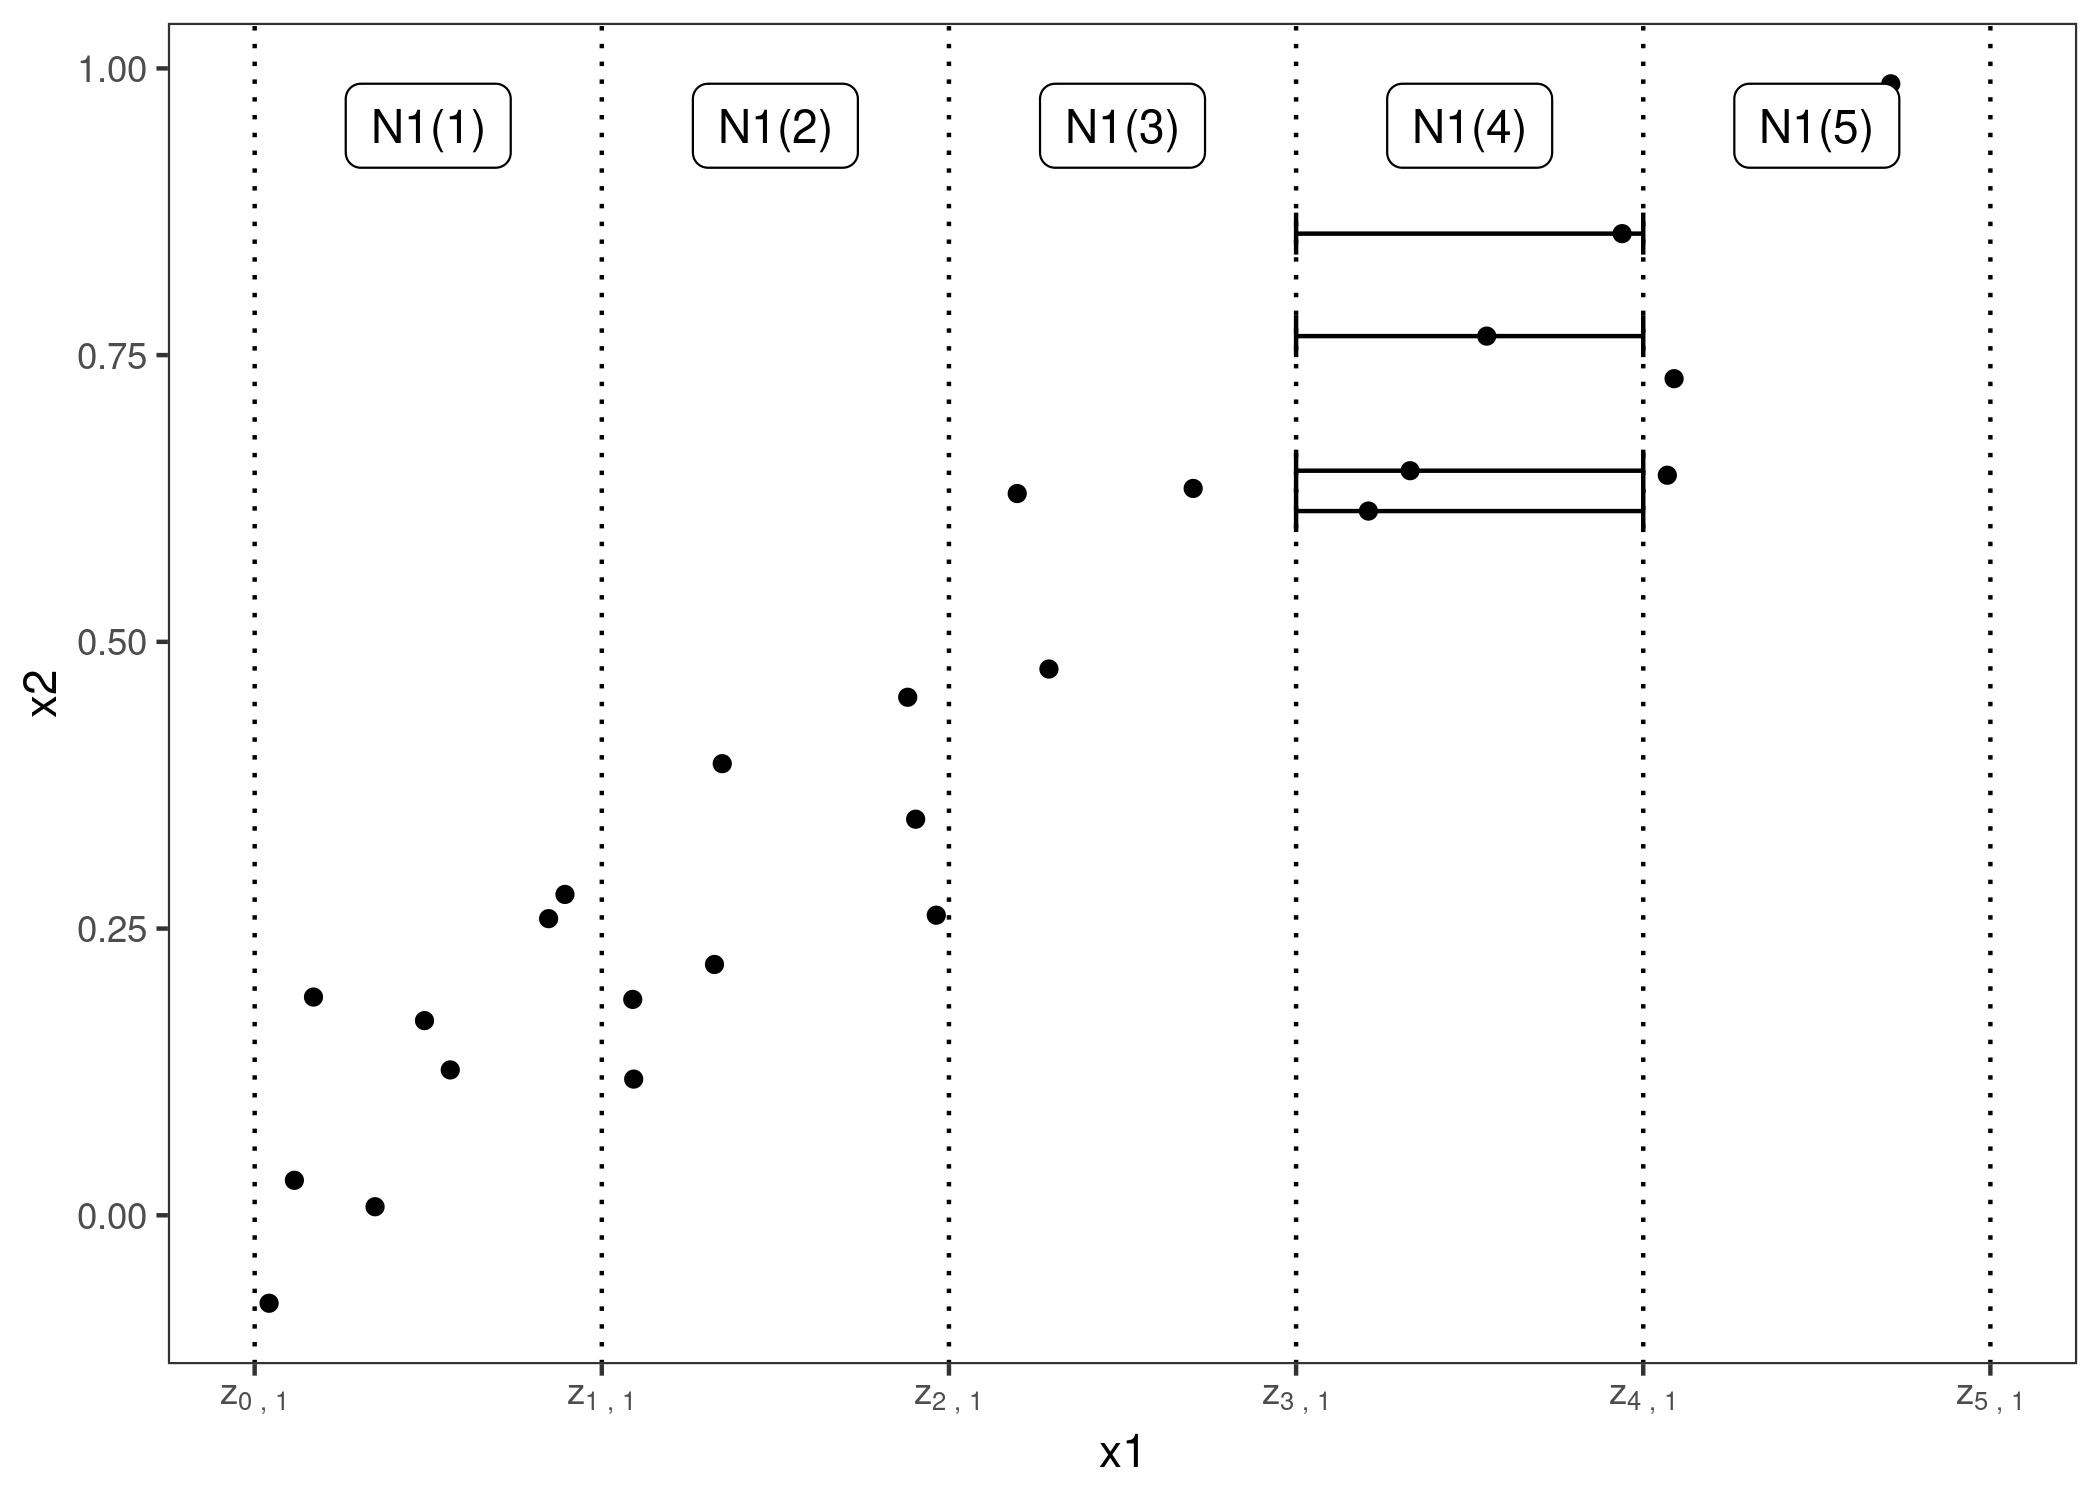
\includegraphics[width=.75\textwidth]{molnar-8-7.jpeg} \\

\scriptsize Source: Molnar, Fig. 8.7
\caption{Illustrative example of ALE computation}
\label{fig:molnar87}
\end{figure}

Consider the illustrative example in Figure~\ref{fig:molnar87}. It shows five neighbourhoods defined for feature $x1$. The four horizontal lines represent the differences in prediction for four observations when the value of $x1$ changes from $Z_{3,1}$ to $Z_{4,1}$, The value of $x2$ is held constant. The four differences are summed to yield the local effect. Local effects are calculated in the same way for the other four intervals in Figure~\ref{fig:molnar87} and then summed. 

To illustrate ALEs, consider the following regression tree, again trained on the bicycle rental count data with the same features and predictors as before.

\begin{samepage}
\begin{pythoncode}
# Train model:
from sklearn.tree import DecisionTreeRegressor
regr=DecisionTreeRegressor(min_samples_leaf=10).fit(x,y)
\end{pythoncode}
\end{samepage}

The PyALE package provides the \texttt{ale} class to calculate the accumulated local effects. They can be plotted for a single feature or for two features. Figure~\ref{fig:ale1} shows the ALE for the temperature feature on bicycle rental counts. The effect of temperature varies across the range of temperature. The two-feature ALE plot is shown in Figure~\ref{fig:ale2} and this also shows a variable impact of the feature combinations on the predicted bicycle rental count. 

\begin{samepage}
\begin{pythoncode}
import matplotlib.pyplot as plt
from PyALE import ale
# Construct the ALE and plot:
ale_effects = ale(X=x, model=regr, \
    feature=['temp'], grid_size=50)
plt.show()
ale_effects = ale(X=x, model=regr, 
    feature=['temp', 'hum'], grid_size=50)
plt.show()
\end{pythoncode}
\end{samepage}

Notably, ALE plots also remove the ''ceteris paribus'' assumption that all other values remain equal. However, instead of overaging over all values of the complement features, as PDPs do, the effects are computed for a local window of complement feature values. This makes ALE suitable for the use with correlated variables. 

\begin{figure}
\centering

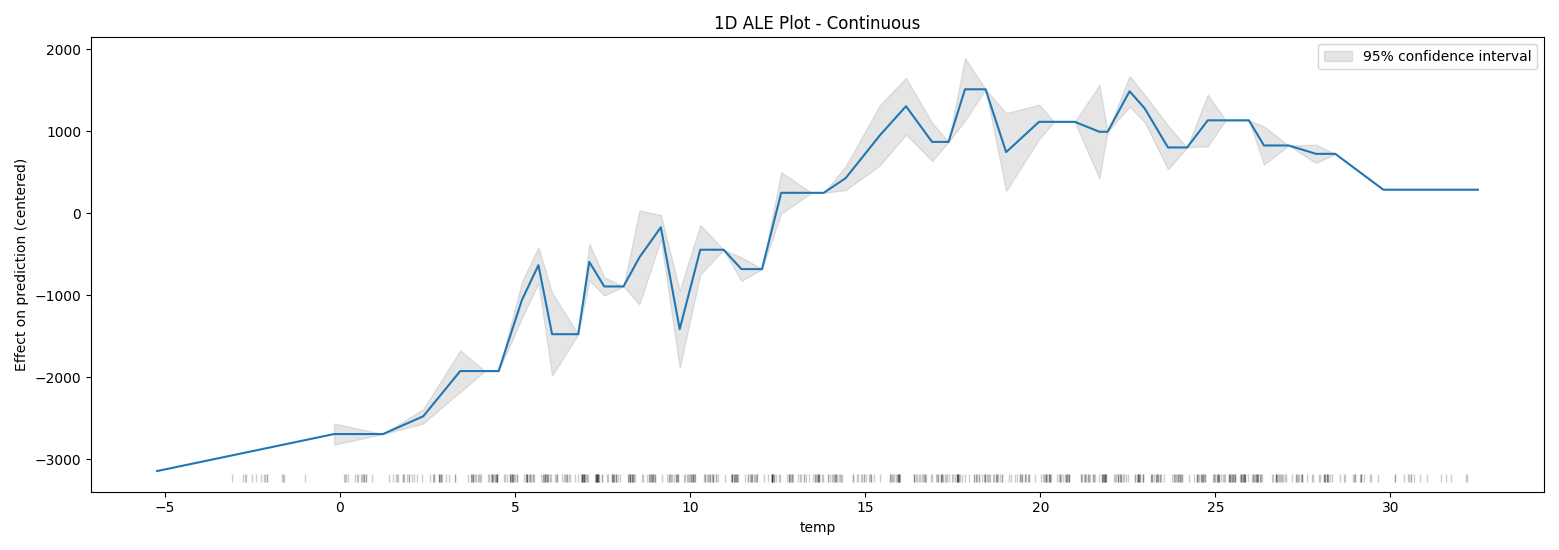
\includegraphics[width=\linewidth]{ale_dtr.png} 
\caption{Example ALE for one feature}
\label{fig:ale1}
\end{figure}

\begin{figure}
\centering

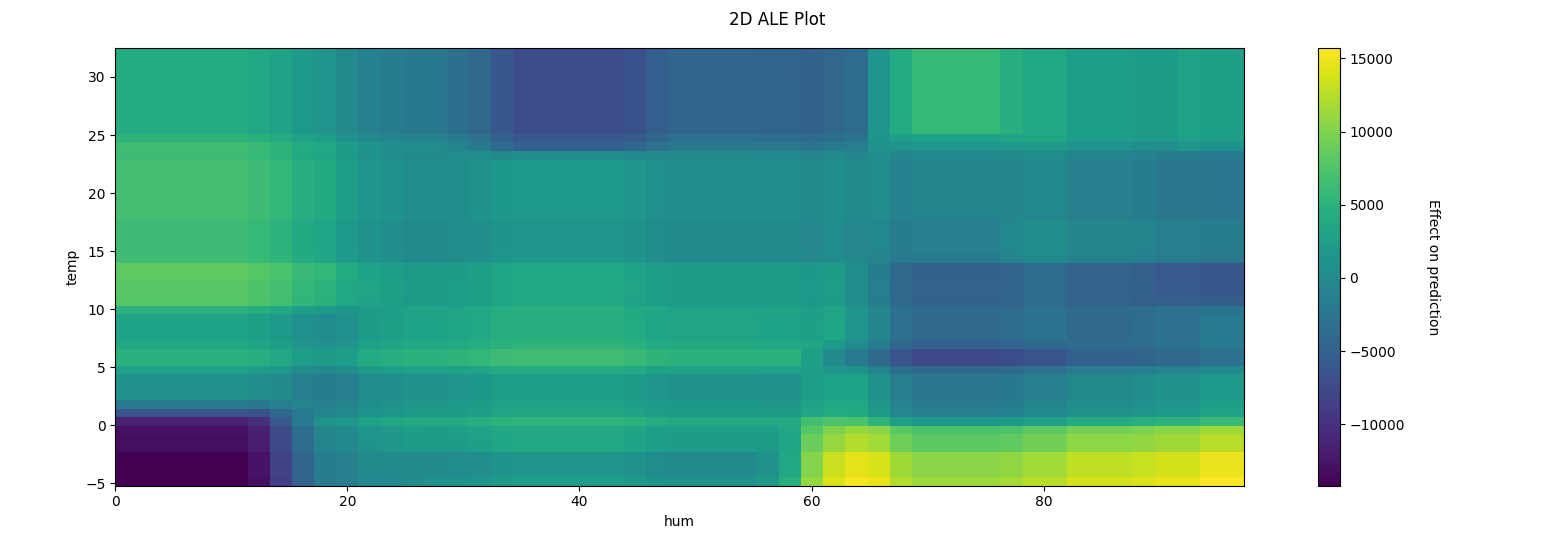
\includegraphics[width=\linewidth]{2d_ale_dtr.png}
\caption{Example ALE for two features}
\label{fig:ale2}
\end{figure}

\FloatBarrier
\subsection{Permutation Feature Importance}

Permutation feature importance\index{Permutation feature importance} assesses the importance of each feature by observing the effect on predictive accuracy when the values of that feature are randomly shuffled. This disrupts the relationship between the feature and the outcome, and a significant drop in model performance indicates that the feature is important for model predictions. The intuition is simple: A feature that has no effect on the prediction outcome can be randomly reshuffled without consequence for the predictive performance of the model.

Permutation feature importance begins by estimating the prediction error (loss function) for the model $L$ on the original data $X$. Permutation feature importance should be calculated on test data, not training data.

\begin{align*}
e^{\text{orig}} = L(y, \hat{f}(X))
\end{align*}

\begin{samepage}
Next, the feature importance is calculated for each feature $j$, using $K$ multiple random shuffles (''permutations'') $k$ of each feature's values:

\begin{itemize}
\item For each feature $j$:
  \begin{itemize}
     \item For each repetition $k$ in $1 \cdots K$:
     \begin{itemize}
        \item Generate permuted data $X^{\text{perm}}_{j, k}$ by permuting (''shuffling'') values of feature $j$
        \item Estimate prediction error of model $L$ for permuted data:
        \begin{align*}e^{\text{perm}}_{j, k} = L(y, \hat{f}(X^{\text{perm}}_{j, k}))\end{align*}
     \end{itemize}
     \item Calculate permutation feature importance: 
     \begin{align*}i_j = e^{\text{orig}} - \frac{1}{K}\sum_k^K e^{\text{perm}}_{j, k}\end{align*}
  \end{itemize}
\end{itemize}
\end{samepage}

The following example again uses the bicycle rental data set. The rental count is used as prediction target, variables other than year and days since 2011 are used as features. A regression tree is fitted with the following Python code block.

\begin{samepage}
\begin{pythoncode}
import pandas as pd
# Prepare data:
d=pd.read_csv('https://evermann.ca/busi4720/bike.csv')
x=pd.get_dummies(d.drop(['yr','days_since_2011'],axis=1))
y=x.pop('cnt')
# Train model:
from sklearn.tree import DecisionTreeRegressor
regr=DecisionTreeRegressor(min_samples_leaf=10).fit(x,y)
\end{pythoncode}
\end{samepage}

The SciKit-Learn package provides the \texttt{permutation\_importance} class to compute feature importance. The \texttt{n\_repeats} parameter specifies the number of permutations to use for each feature. For simplicity of exposition, the permutation feature importance is calculated here using the training data, but practical applications should use independent test data for this. The second line in the code below sorts the permutation feature importances by their mean for later plotting.

\begin{samepage}
\begin{pythoncode}
from sklearn.inspection import permutation_importance
# Calculate permutation feature importance and sort them
r = permutation_importance(regr, x, y, n_repeats=30)
r_idx = r.importances_mean.argsort()
\end{pythoncode}
\end{samepage}

The feature importances can be easily visualized using the following Python code. The resulting graph is shown in Figure~\ref{fig:pfi}. The graph shows that temperature has the greatest importance, followed by humidity and windspeed. Many features have little or no impact on the prediction outcome.

\begin{samepage}
\begin{pythoncode}
import matplotlib.pyplot as plt
# Produce a plot of sorted feature importance:
fig, ax = plt.subplots()
ax.boxplot(r.importances[r_idx].T,vert=False,labels=x.columns[r_idx])
ax.axvline(x=0, color="k", linestyle="--")
plt.show()
\end{pythoncode}
\end{samepage}

\begin{figure}
\centering

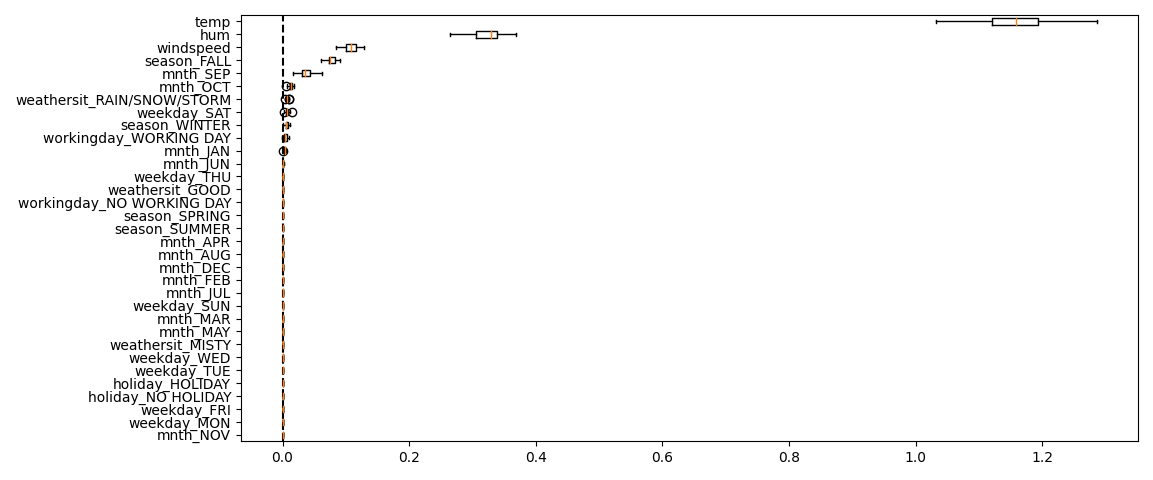
\includegraphics[width=.75\textwidth]{pfi_tree.png} \\
\caption[Permutation feature importance plot]{Permutation feature importance plot. Uncertainty represents variation of multiple permutations}
\label{fig:pfi}
\end{figure}

\subsection{Global Surrogate Models}

Global surrogate interpretation models\index{Global surrogate interpretation model} are interpretable models that are trained to approximate the predictions of a complex model. By training a simpler model (like a decision tree or linear regression model) to mimic the behavior of a more complex model, insights can be gained into how the complex model makes decisions, providing an interpretable approximation of its decision-making process. Intuitively, the predictions of the complex model are the prediction targets of the simpler surrogate model, that is, the simple surrogate model should predict the predictions (rather than the original target values).

Doing this in practice is simple. For example, the following Python code trains a neural network regression model with two hidden layers and ReLU activation function on the bicycle rental data set. The model is then used to predict values for the training observations.

\begin{samepage}
\begin{pythoncode}
# Example 'black box' model
from sklearn.neural_network import MLPRegressor
regr = MLPRegressor((4, 2,), max_iter=10000)
regr.fit(x, y)
preds = regr.predict(x)
\end{pythoncode}
\end{samepage}

In the second step, a simpler surrogate model is used to predict the predictions. The following example uses a linear regression model fitted using ordinary least squares. As noted above, the absolute value of the $t$ statistic in the fitted OLS model serves as an indication of feature importance in this surrogate model. The summary results indicate that the surrogate model has an $R^2$ value of $0.995$, that is, it explains the predictions of the complex model (not the original targets!) very well. 

\begin{samepage}
\begin{pythoncode}
from statsmodels.api import OLS
OLS(preds, x).fit().summary()
\end{pythoncode}
\end{samepage}

\begin{table}
\centering
%\footnotesize
\renewcommand{\arraystretch}{1.1}
\begin{tabular}{l|l} \hline
\multicolumn{2}{c}{\textbf{PDP/ICE}} \\ \hline
Intuitive & Limited number of features \\
Clear interpretation & Assumes feature independence \\
Easy to implement & \\ \hline
\multicolumn{2}{c}{\textbf{ALE}} \\ \hline
Unbiased for correlated features & Local interpretation only\\
Clear interpretation & ALE may differ from linear coefficients\\ 
Faster to compute than PDP & No ICE curves \\
& Unstable for large number of intervals \\  \hline
\multicolumn{2}{c}{\textbf{PFI}} \\ \hline
Clear interpretation & Linked to model error \\
Concise, global measure & Requires access to true targets \\
Does not require retraining & May be biased for correlated features \\
Takes into account all interactions & \\ \hline
\multicolumn{2}{c}{\textbf{Global Surrogate Models}} \\ \hline
Flexible & Conclusions about model, not data \\ 
Intuitive & Unclear cut-off for goodness of fit \\
R-squared measure for fit & \\ \hline
\end{tabular}
\caption[Strengths and weaknesses of global model-agnostic methods]{Strengths and weaknesses of different global model-agnostic methods}
\label{tab:summaryglobalmethods}
\end{table}

Table~\ref{tab:summaryglobalmethods} summarizes the strengths and weaknesses of the different global model-agnostic methods for interpretable machine learning discussed in this section.

\section{Local Model-Agnostic Interpretation Methods}

Local model-agnostic interpretable methods\index{Local model-agnostic interpretable method} aim to provide explanations for individual predictions or cases, regardless of the overall model's complexity or opacity, offering insights into specific decision points rather than a model's global behavior. This section presents two widely-used methods that each address the challenge of interpretability from a different perspective.

\subsection{Local Interpretable Model-agnostic Explanations (LIME)}

The intuition behind LIME\index{Local interpretable model-agnostic explanations}\index{LIME|see{Local interpretable model-agnostic explanations}} is that while it may be difficult or impossible to explain an entire complex model globally, it is possible to approximate and explain its behavior locally. LIME generates these local explanations by perturbing (''shuffling'') the feature values of the input observations to create a new dataset consisting of ''synthetic'' observations around an observation of interest. The responses of the complex model to these synthetic observations are then used to train a simpler, interpretable model, such as a linear regression or decision tree. This local surrogate model aims to capture how the original complex model behaves in the vicinity of the specified observation, providing insights into which features significantly influence the output and how they do so. LIME can be applied to any model type without any changes to the underlying algorithms. 

LIME follows these steps:

\begin{enumerate}
\item Fit the complex model $f$
\item Choose an instance $x$ of interest for which the prediction is to be explained
\item Transform the instance into a binary vector indicating the presence or absence of ''interpretable components''. Interpretable components are feature values, not features themselves.
\item Create a neighbourhood of $n$ observations around $x$ by perturbing interpretable components (sampling presence or absence of interpretable components randomly from [0,1]).
\item Use the fitted complex model $f$ to create predictions for the generated neighbourhood of observations.
\item Weight the generated observations around $x$ by a weight kernel $\pi_g$ based on their distance to the instance $x$.
\item Sample a number of observations according to their weight.
\item Fit a local surrogate, interpretable model $g$ to the sampled observations, using a set of $k$ features, that minimizes the discrepancy $\mathcal{L}$ between $g$ and the complex original model $f$.
\begin{itemize}
   \item The usual local surrogate model is a ridge regression model.
   \item The $k$ features are identified by forward selection, by LASSO, or simply by selecting $k$ features with the highest regression weights.
\end{itemize}
\end{enumerate}

In principle, LIME aims to identify the explanation model as that local surrogate model $g$ that minimizes the sum of the discrepancy between surrogate and original model plus a complexity penalty $\Omega(g)$ for the surrogate model:

\begin{align*}
\xi(x) = \operatorname*{argmin}_{g \in G} \; \mathcal{L} (f, g, \pi_x) + \Omega(g)
\end{align*}

However, in practice, as noted in the LIME procedure steps, the analyst must select the number of features and the type of local surrogate model. LIME only minimizes the discrepancy to the complex model; the complexity is determined by the analyst.

Figure~\ref{fig:molnar95} illustrates the principles behind LIME. The top left panel shows a classification problem with two predictors $x1$ and $x2$ and a somehwat complicated decision boundary. 

\begin{figure}
\centering
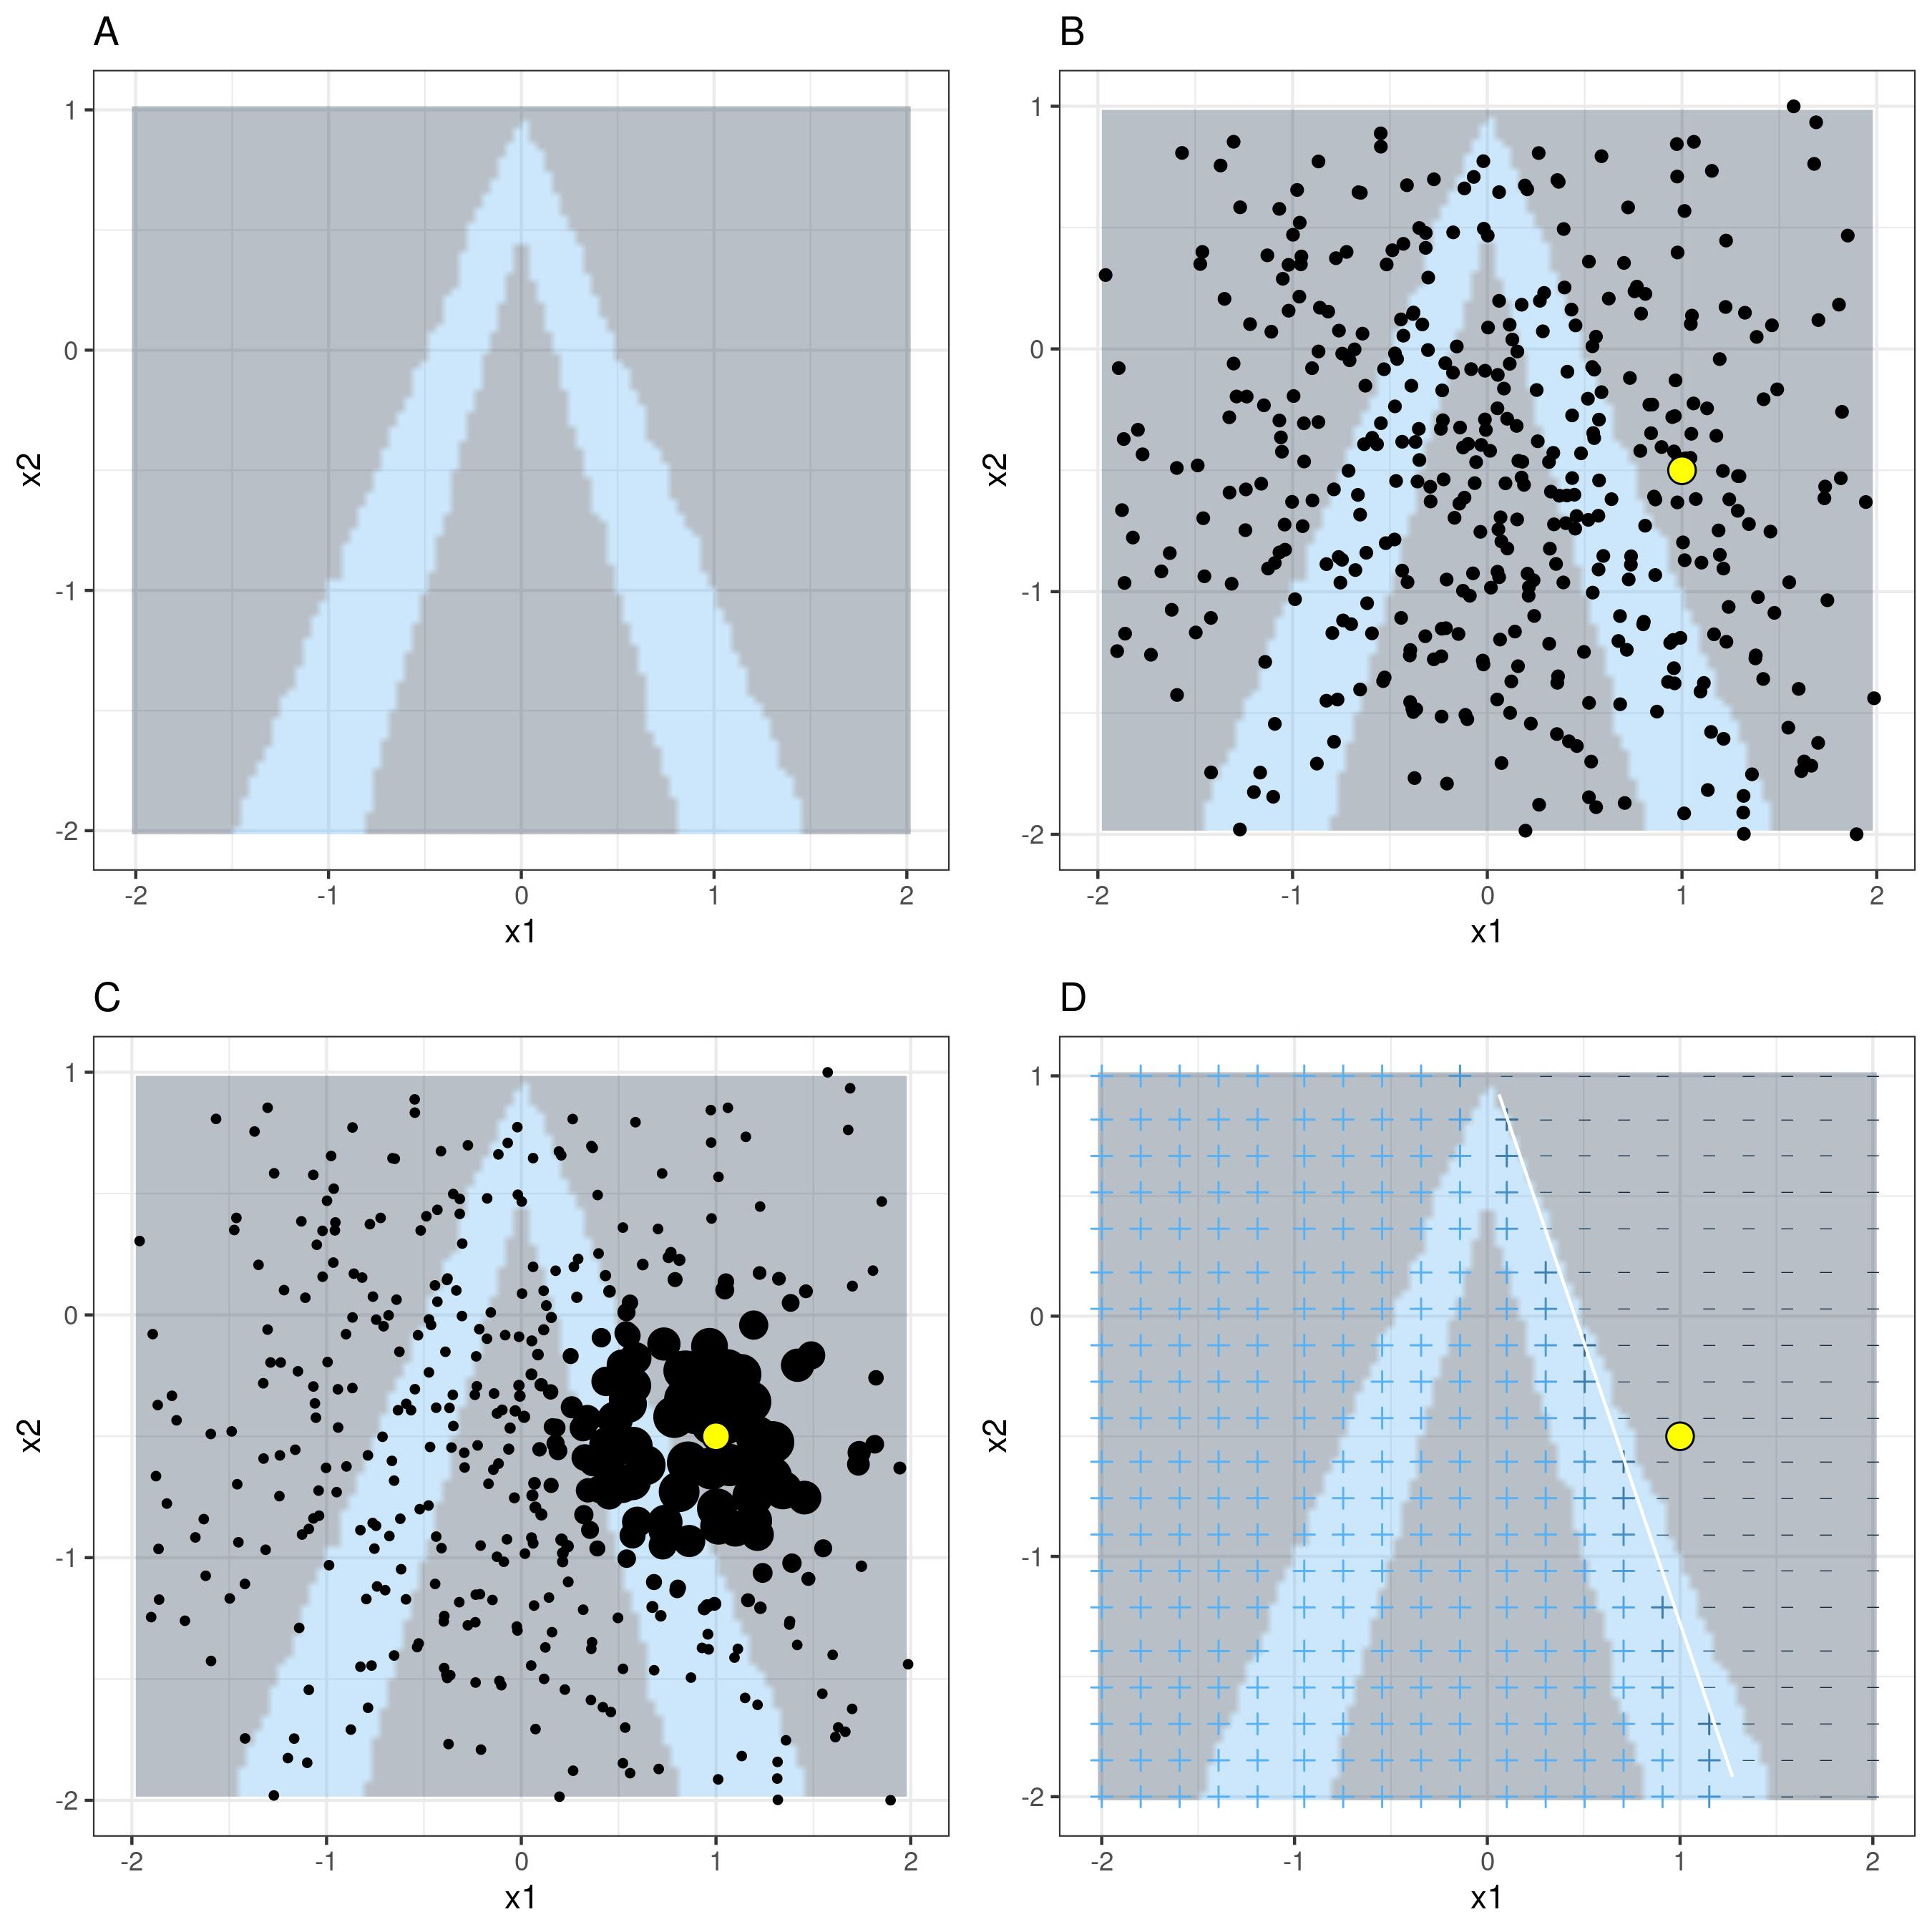
\includegraphics[width=0.75\textwidth]{molnar-9-5.jpeg} \\

\scriptsize Source: Molnar Figure 9.5
\caption{Illustration of LIME}
\label{fig:molnar95}
\end{figure}

The top right panel highlights the target observation $x$ in yellow and shows the observations created by perturbing the feature values as black dots. 

The bottom left panel indicates the weighting of observations in the neighbourhood, bigger dots indicate higher weights. This weighting is induced by the distance function\index{Distance function} and the weight kernel\index{Weight kernel}. The distance function specifies how distances in the feature space are measured, for example Euclidean, Chebyshev or other metrics. The weight kernel uses the distances to assign weights. For example, a Gaussian kernel will assign weights according to a normal distribution density function, and an exponential kernel will assign weights according to the exponential of the distance, with higher weights for smaller distances and lower weights for larger distances. 

The bottom right panel shows the class predictions of the simple surrogate model that has been fitted to the weighted samples. The white line shows the linear decision boundary of the surrogate model, the superimposed plus and minus signs the predictions of the surrogate model. The local surrogate model is quite accurate for values in the vicinity of the focal observation, but not very good for points far away from it.

Figure~\ref{fig:molnar96} illustrates the strong dependence of LIME results on the kernel, in particular the width of the kernel. The ''X'' marks the focal observation, and the graph plots the values predicted by the complex model against the values predicted by the simple model for different kernel widths. The point that Figure~\ref{fig:molnar96} makes is that not only the strength but also the sign or direction of the relationship between the predictions of the two models can change, depending on the choice of kernel. 

\begin{figure}
\centering

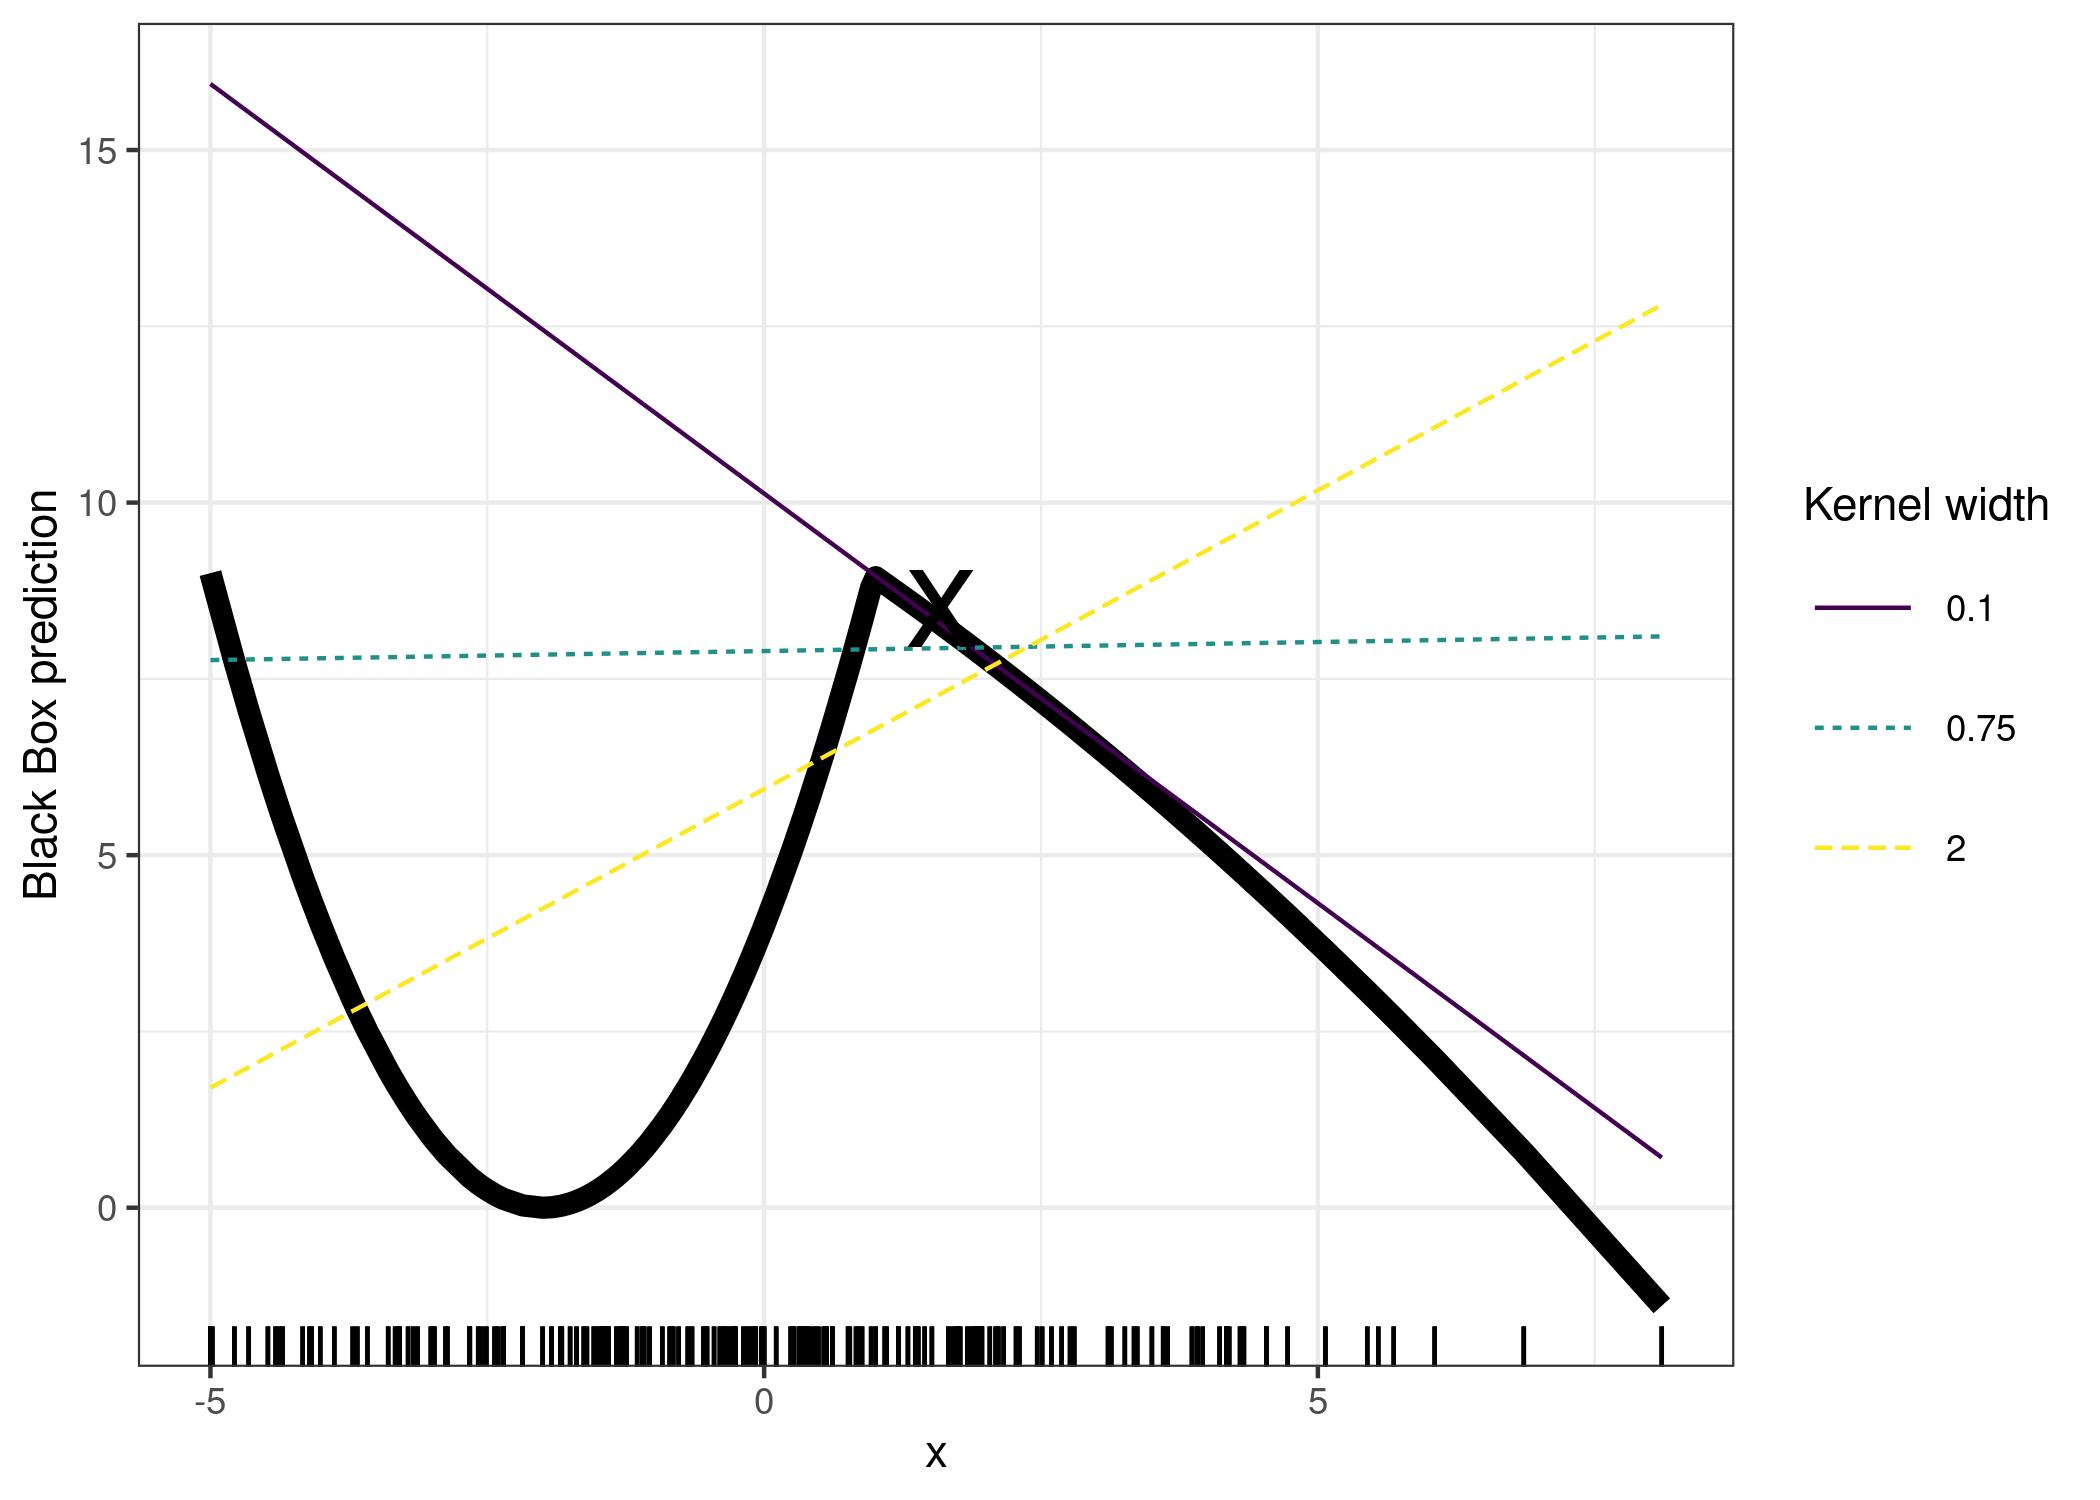
\includegraphics[width=.75\textwidth]{molnar-9-6.jpeg} \\

\scriptsize Source: Molnar Figure 9.6
\caption{LIME results depend on choice of weight kernel}
\label{fig:molnar96}
\end{figure}

The following Phython code block uses LIME to provide an explanation for the predictions of a decision tree classifier. 

\begin{samepage}
\begin{pythoncode}
import sklearn.tree
# Using a deep decision tree as black box model
dt = sklearn.tree.DecisionTreeClassifier(max_depth=8)
dt.fit(x, y)
\end{pythoncode}
\end{samepage}

The \texttt{lime} package provides the \texttt{LimeTabularExplainer} for regular datasets consisting of rows and columns. LIME can also be applied to other types of data such as images, see below.

\begin{samepage}
\begin{pythoncode}
import lime, lime.lime_tabular
# Create the explainer
explainer = lime.lime_tabular.LimeTabularExplainer(
    x.to_numpy(), 
    feature_names=x.columns, 
    discretize_continuous = True, 
    mode='regression', 
    verbose=True)
\end{pythoncode}
\end{samepage}

With the explaining model created, specific data instances can be explained using the \texttt{explain\_instance()} method. The following example code explains the prediction for the 8th instance in the training data set that is generated by the \texttt{predict()} method of the regression tree object. The local neighbourhood is created with $n=1000$ samples, the explanation is limited to $k=5$ features, and the distance between observations for weighting them is determined by the Euclidean distance.

\begin{samepage}
\begin{pythoncode}
# Explain instance number 7
exp = explainer.explain_instance( 
    x.to_numpy()[7], 
    dt.predict, 
    num_features=5, 
    num_samples=1000, 
    distance_metric='euclidean')
# Show weights as text and visualize
exp.as_list()
exp.as_pyplot_figure().show()
# Show complete explanation
exp.save_to_file('lime_explanation.html')
\end{pythoncode}
\end{samepage}

The results indicate the contribution of each feature value to the prediction. Note that continuous variables like temperature and windspeed have been discretized at various boundaries to form interpretable components. The visualizations in Figure~\ref{fig:limecontribs} and Figure~\ref{fig:limeexplanation} shows those contributions as well. 

\begin{samepage}
\begin{textcode}
[('temp <= 7.84', -1738.6611673589232), 
 ('mnth_MAR <= 0.00', 640.903016649792), 
 ('weekday_THU <= 0.00', -532.3918204920352), 
 ('windspeed > 15.63', 493.90993722141997), 
 ('season_SPRING <= 0.00', -333.38496260796086)]
\end{textcode}
\end{samepage}

Figure~\ref{fig:limeexplanation} consists of three parts. The left panel shows the prediction for this instance, $959$ on the scale between the minimum ($431$) and maximum ($7403$). The right panel shows the actual feature values for the observation in table form. The center panel (which is identical to Figure~\ref{fig:limecontribs}) shows the negative and positive contribution of each interpretable component. For example, the contribution of $temp <= 7.84$ is $-1738.66$. This means that if the temperature were \emph{not} equal to or below 7.84 degrees, the prediction would be $1738$ higher than it is, that is, it would be $2697$. Similarly, the feature $mnth MAR <= 0.00$ contributes positively to the prediction ($640.90$). This means that if the month were March, the prediction would be $640.00$ lower than it is. 

\begin{figure}
\centering

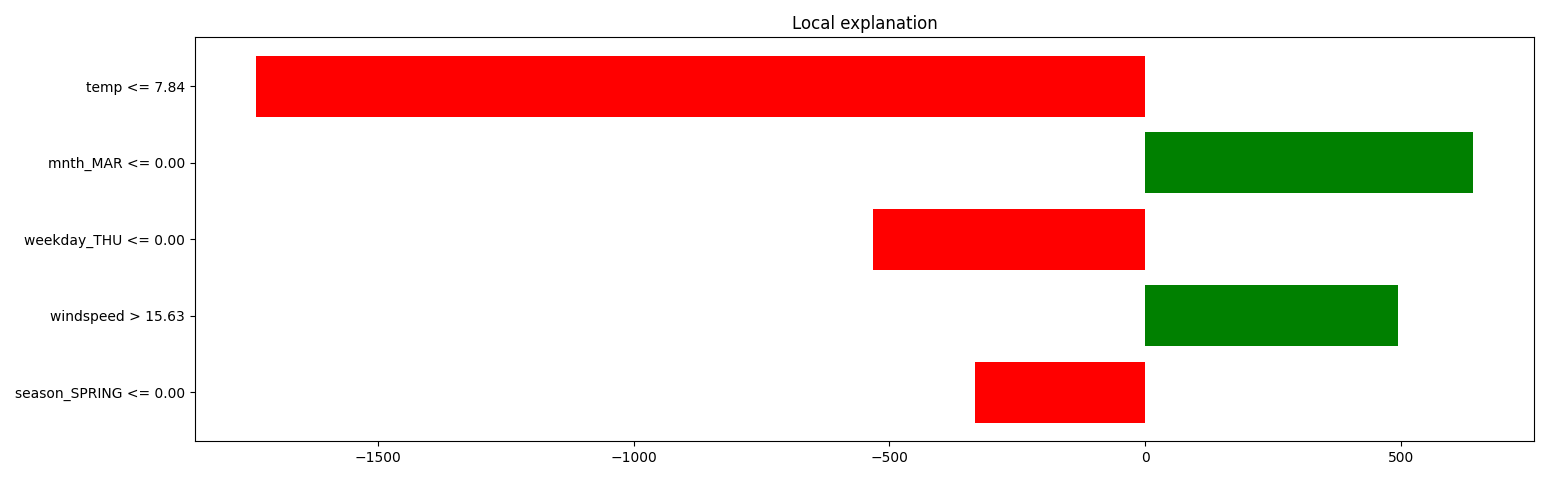
\includegraphics[width=\textwidth]{lime_dt.png}
\caption{Weights of the LIME local surrogate model}
\label{fig:limecontribs}
\end{figure}

\begin{figure}
\centering

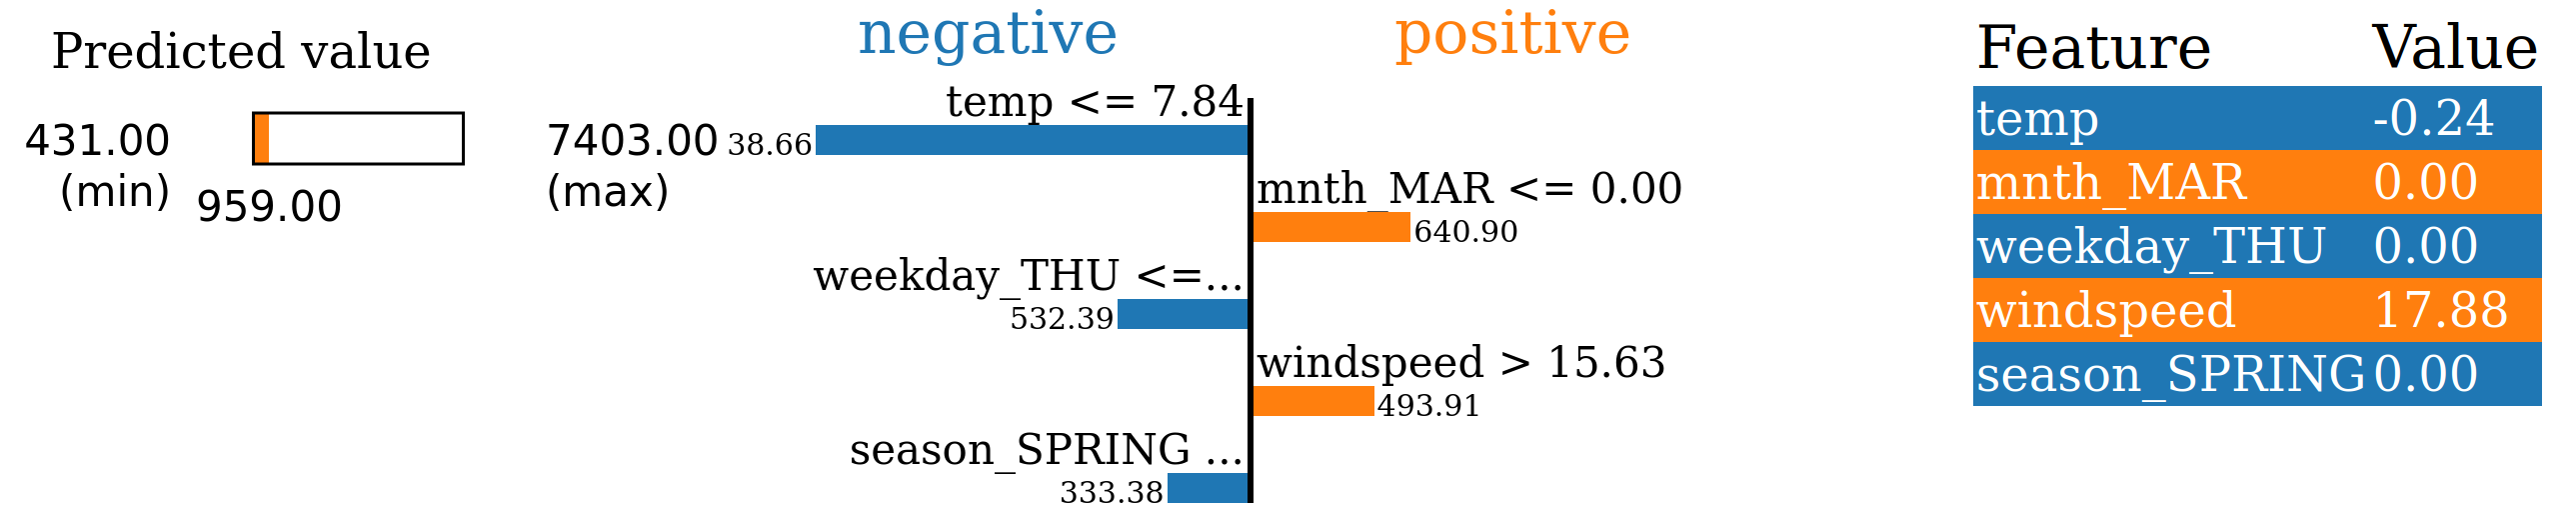
\includegraphics[width=\textwidth]{lime_explanation.png}
\caption{LIME results for explaining a specific instance}
\label{fig:limeexplanation}
\end{figure}

LIME can also be used on other models such as image or text classification models. For example, Figure~\ref{fig:molnar98} shows the contributions of individual pixels of an image to the classification of that image. The left panel shows the original image, the middle panel the contributions for the label ''bagel'' and the right panel the contributions for the label ''strawberries''. 

\begin{figure}
\centering
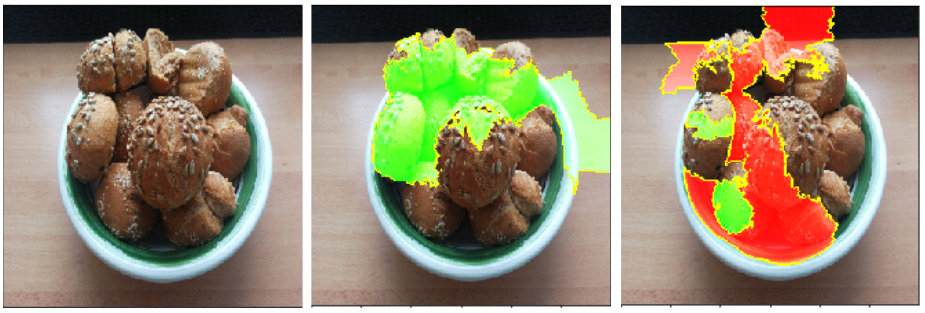
\includegraphics[width=\textwidth]{molnar-9-8.png} \\

\scriptsize Molnar, Figure 9.8
\caption{LIME explanations for image classification}
\label{fig:molnar98}
\end{figure}

\begin{tcolorbox}[colback=code]
\small
Further information on LIME, including many examples, can be found at the website for the Python package\footnote{\url{https://github.com/marcotcr/lime}}. More details on the theoretical foundation and principles of LIME can be found in the original paper\footnote{\url{https://arxiv.org/abs/1602.04938}}.
\normalsize
\end{tcolorbox}

\subsection{Shapley Additive eXplanations (SHAP)}

Developed from the Shapley value -- a concept from cooperative game theory originally used to determine the fair distribution of payoffs among players -- SHAP applies this framework to the domain of machine learning, offering a theoretically sound approach to understanding model behavior. SHAP treats each feature value as a ''player'' in a game where the ''payout'' is the prediction itself. The Shapley value calculates the average contribution of each feature value across all possible combinations of feature values, providing a detailed view of how features interact and influence the model's output. This approach not only yields a measure of global feature importance and local feature value importance, but also provides a way to understand the direction and magnitude of each feature's impact on the prediction. SHAP is model-agnostic and can be applied to any machine learning model, from simple linear regressors to deep neural networks. 

The main motivation in SHAP is the question of how much does a specific value $x_j$ of feature $j$ contribute to the overall prediction, when compared to the average prediction. As in LIME, the focus is on values of features, not the features themselves. In cooperative game theory, players cooperate in a coalition\index{Coalition} with other players and receive a certain profit from this cooperation. Shapley values are named after Lloyd Shapley who developed this concept in 1951 and received the Nobel prize in Economics for his work in 2012. Shapley values are a method for assigning fair payouts to the coalition's players depending on their contribution to the total payout. 

Formally, the Shapley value $\phi_i$ of player $i$ is defined as\index{Shapley value}:

\begin{align*}
\phi_i(v) = \frac{1}{n} \sum_{S \subseteq N \setminus \{i\}} \binom{n-1}{|S|}^{-1} \left[ v(S \cup \{i\}) - v(S)\right]
\end{align*}

where $v(.)$ is the value function that describes the payout received in a game\index{Payout}. The term $v(S \cup \{i\}) - v(S)$ is the marginal contribution of player $i$ to a coalition of players $S$, that is, the difference in payout received by the coalition $S$ plus the player $i$ and the payout received only by the coalition $S$, without player $i$. 

The binomial coefficient $\binom{n-1}{|S|}$ represents the number of possible ways to form a coalition of size $|S|$ of the set $N \setminus \{i\}$ of $n-1$ players (set $N$ without player $i$). The marginal contribution is divided by this term. 

The sum is taken over all all possible coalitions of the set $N$ of players minus the player $i$. The sum is then divided by the number of players $n$.

Shapley values have some key theoretical properties that together ensure they describe a fair allocation of value or contribution to each player:

\begin{itemize}
    \item \emph{Efficiency:}
    The efficiency property states that all gains from cooperation are distributed among the players. Mathematically, this means the sum of the Shapley values for all players equals the total value (or payoff) that the coalition of all players achieves together. This ensures that the Shapley value captures the entire surplus generated by the group, leaving no residual value unallocated.

    \item \emph{Symmetry:}
    The symmetry property ensures that if two players contribute equally to any coalition they are both members of, they receive the same proportion of the payoff. In other words, the Shapley value is identical for symmetric players, reflecting the principle of fairness in that contributions are rewarded equally without bias to factors unrelated to the contribution.

    \item \emph{Additivity (or Linearity):}
    Additivity is a property where the Shapley value of a game can be derived by summing the Shapley values of two separate games if a player's value in a combined game is the sum of their values in these separate games. This property allows for straightforward aggregation of separate contributions, simplifying the analysis and computation in more complex scenarios.

    \item \emph{Dummy (or Null Player):}
    A dummy (or null) player does not contribute to any coalition, i.e., the addition of this player does not change the value of any coalition. The dummy player property ensures that such a player receives a Shapley value of zero. This ensures that only contributors to a game's outcome are rewarded, maintaining the integrity of the allocation process.
\end{itemize}

In the context of interpretable machine learning, the players in a coalition are specific values of features (\emph{not the feature themselves}). A coalition is a combination of different feature values. The presence of a feature value in a coalition means that the value of that feature is known and fixed. When a feature is not present in a coalition with a specific value, its value is unknown. Determining the payout requires integrating or marginalizing over all values of those features $1 \ldots p$ that are not in a coalition $S$.

\begin{align*}
v_x(S) = \idotsint_\Bbb{R} \hat{f}(x_1, \ldots, x_p) d\Bbb{P}_{x \not\in S} - E_x(\hat{f}(X))
\end{align*}

This is clearly expensive to compute in practice and is therefore generally approximated by randomly permuting values (similar to how LIME constructs its local neighbourhood of observations) and then sampling the different possible coalitions from these permuted values. 

\vspace{2\baselineskip}

\begin{wrapfigure}{l}{1in}
\begin{center}

\includegraphics[height=.45in]{shap_logo.png}
\end{center}
\end{wrapfigure}
Shapley Additive eXplanations (SHAP) is a Python package developed by authors of the paper that introduced Shapley values to interpretable machine learning\footnote{\url{https://arxiv.org/abs/1705.07874}}. A thorough documentation, including an easy to read introduction and many examples are available\footnote{\url{https://shap.readthedocs.io/en/latest/index.html}}, as well as the Python code for the implementation and multiple tutorial\footnote{\url{https://github.com/shap/shap}}. The remainder of this section illustrates the basic usage of SHAP.

This example uses a data set on California house prices that is part of the SHAP package. The target variable are house values in various districts, and predictors inlcude median income, number of rooms, population, and similar variables. To illustrate the basic use of SHAP, this example fits a simple linear regression model to the data.

\begin{samepage}
\begin{pythoncode}
import sklearn
import shap
# Fit a simple regression model
X, y = shap.datasets.california(n_points=1000)
model = sklearn.linear_model.LinearRegression().fit(X, y)
\end{pythoncode}
\end{samepage}

The SHAP \texttt{Explainer} object is constructed using the fitted model's prediction function and the training data set. The explainer object can then be used to explain predictions in the same or another data set, e.g. just a for a single new observation, or for the test or validation data set. The following Python code block illustrates this usage:

\begin{samepage}
\begin{pythoncode}
# Create the Explainer object:
explainer = shap.Explainer(model.predict, X)
# Compute the SHAP values:
shap_values = explainer(X)
\end{pythoncode}
\end{samepage}


The SHAP package provides different ways to visualize individual predictions. The \emph{barplot} in Figure~\ref{fig:shapbar1} shows the importance of feature values (\emph{not the importance of features!}) for an individual prediction, generated from the running example using the following Python code:

\begin{pythoncode}
shap.plots.bar(shap_values[20])
\end{pythoncode}

\begin{figure}
\centering

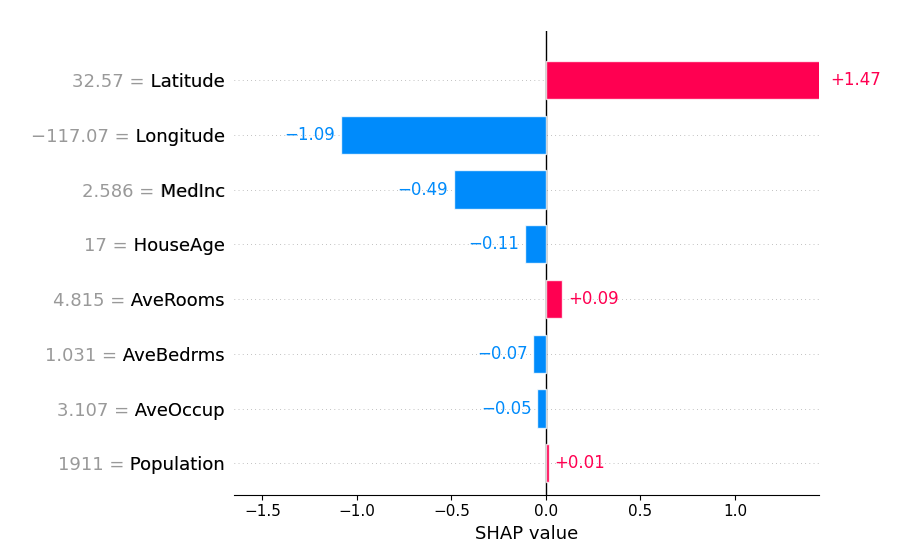
\includegraphics[height=2in]{shap_barplot1.png}
\caption{SHAP barplot for an individual prediction}
\label{fig:shapbar1}
\end{figure}

For example, the fact that the house age is $17$ contributes negatively to the prediction, whereas the fact that the avarage number of rooms of houses in the district is $4.815$ contributes positively.

By averaging over all instances and their feature values, SHAP values can be aggregated to show the importance of the features themselves, shown in the bar plot in Figure~\ref{fig:shapbar2}, generated from the running example using the following Python code:

\begin{pythoncode}
shap.plots.bar(shap_values)
\end{pythoncode}

The graph shows that latitude and longitude are the most important features, that is, their values on average contribute positively to the prediction. 

\begin{figure}
\centering

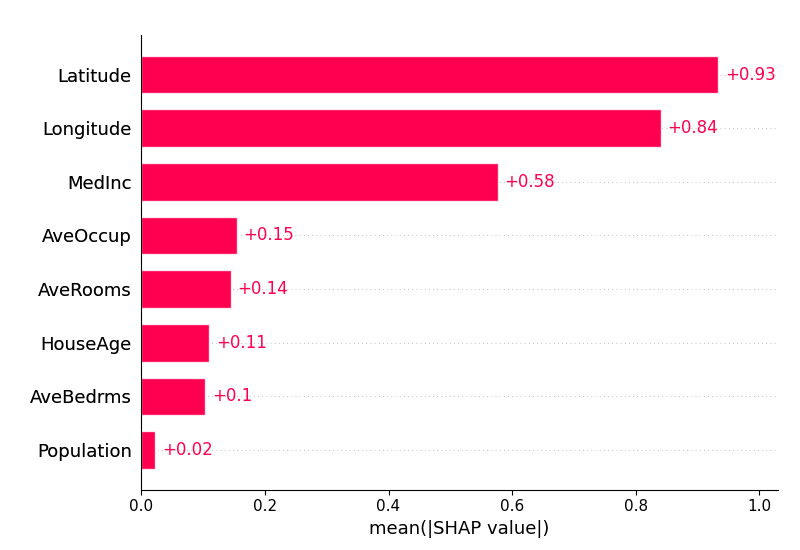
\includegraphics[height=2in]{shap_barplot2.png}
\caption{SHAP barplot of mean SHAP values for feature importance}
\label{fig:shapbar2}
\end{figure}

\emph{Waterfall plots} such as the one in Figure~\ref{fig:shapwaterfall} explain how feature values combine to produce an individual prediction. In that figure, latitude being $32.57$ contributes positively to the house price prediction, whereas longitude being $-117.07$ contributes negatively, etc. The total sum of contributions is the expected house price, shown at the very bottom of the waterfall plot. The waterfall plot was generated by the following Python code:
 
\begin{pythoncode}
sha.plots.waterfall(shap_values[20])
\end{pythoncode}

\begin{figure}
\centering

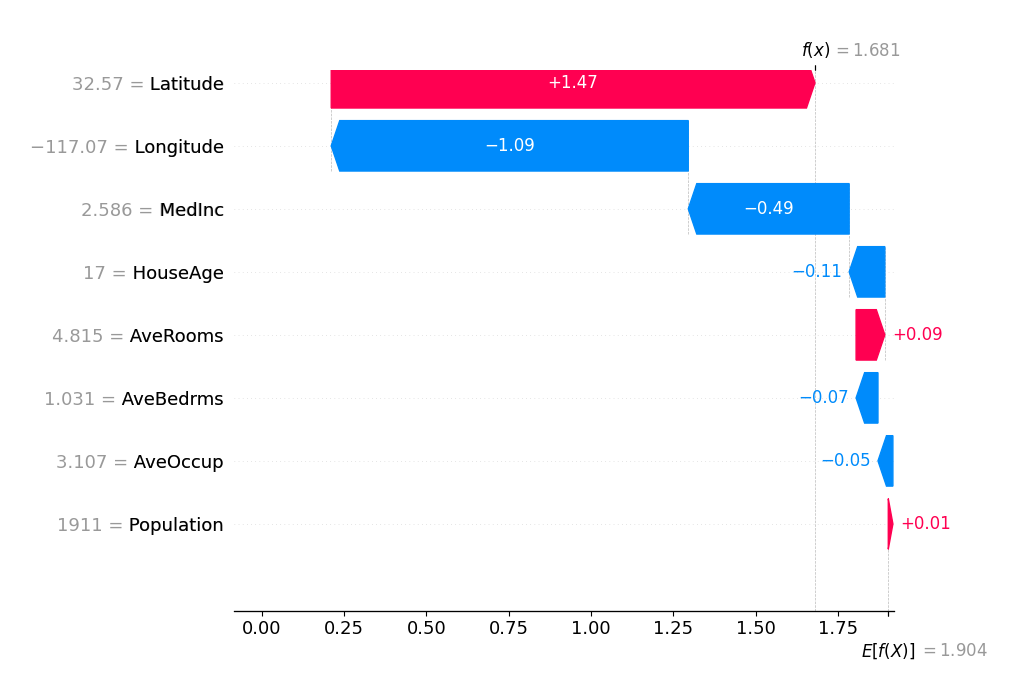
\includegraphics[height=2in]{shap_waterfall1.png}
\caption{SHAP waterfall plot for an individual prediction}
\label{fig:shapwaterfall}
\end{figure}


\emph{Beeswarm plots}, such as the one in Figure~\ref{fig:shapbeeswarm} explain all feature values for all instances (represented by a dot). Each dot is particular feature value that occurs in the data. Dots are colour-coded to indicate whether that feature value makes a positive or negative contribution. Figure~\ref{fig:shapbeeswarm} shows that the median district income feature has a lot of feature values in the data set that contribute negatively, and a few values that make a highly positive contribution. Figure~\ref{fig:shapbeeswarm} was generated using the following Python code.

\begin{pythoncode}
shap.plots.beeswarm(shap_values)
\end{pythoncode}

\begin{figure}
\centering

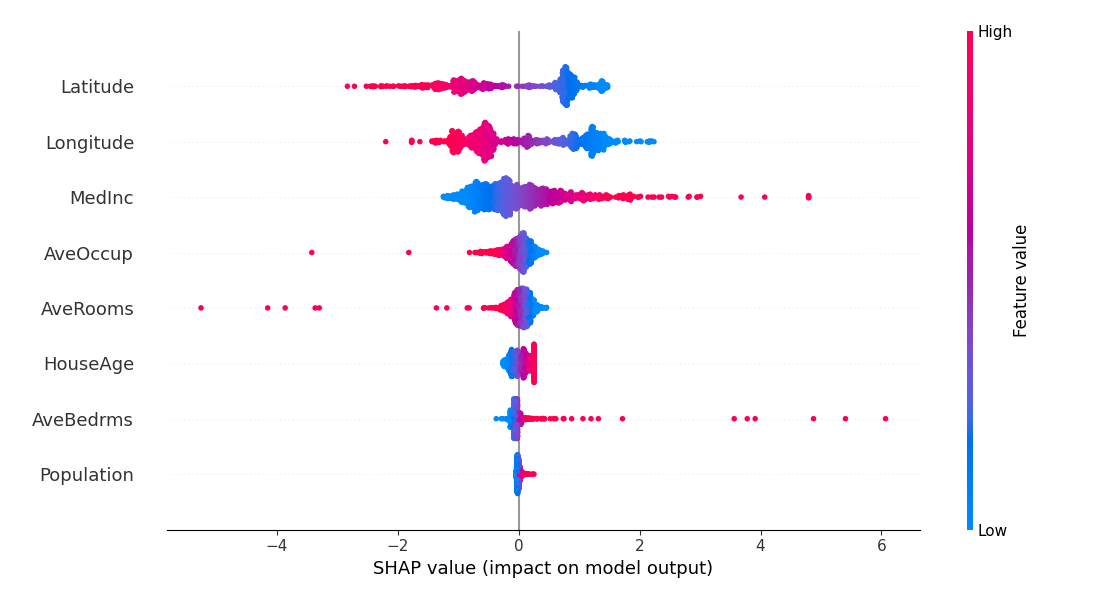
\includegraphics[height=2in]{shap_beeswarm1.png}
\caption{SHAP beeswarm plot}
\label{fig:shapbeeswarm}
\end{figure}


The \emph{heatmap plot} in Figure~\ref{fig:shapheatmap} shows the SHAP values of feature values for all instances, and shows model prediction and global feature importance in the top and right rugs of the figure. Observations are ordered left to right. The bar plot in the right rug is the same as the feature importance bar plot in Figure~\ref{fig:shapbar2}. The figure shows clearly how some values of median district income contribute highly positively to predicted house prices, whereas some values of latitude appear to contribute negatively the predicted house price. Figure~\ref{fig:shapheatmap} was generated using the following Python code:

\begin{pythoncode}
shap.plots.heatmap(shap_values)
\end{pythoncode}

\begin{figure}
\centering

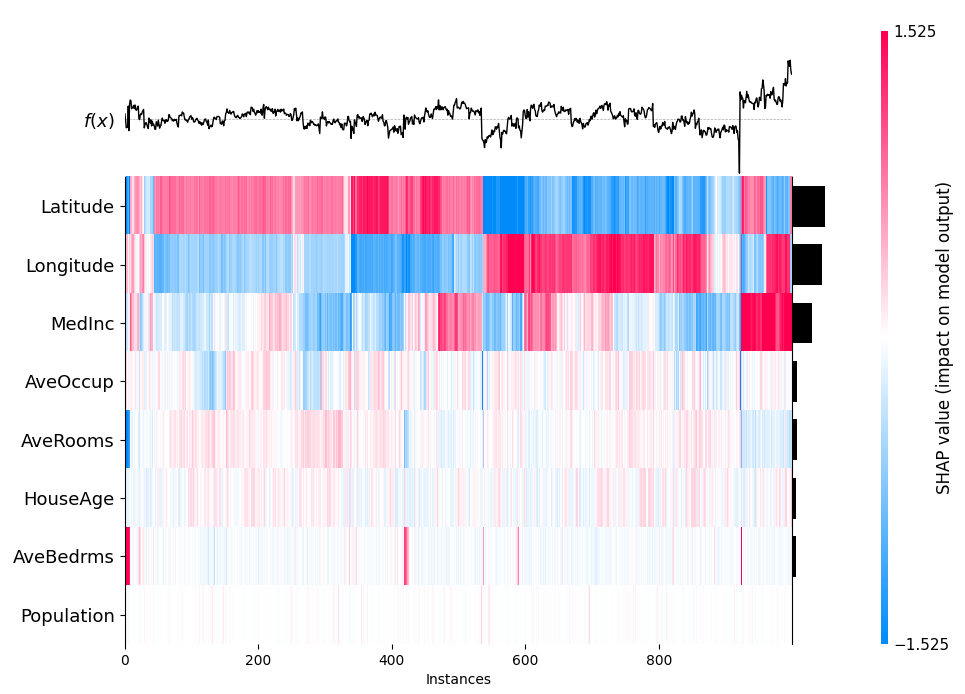
\includegraphics[height=2in]{shap_heatmap1.png}
\caption{SHAP heatmap plot}
\label{fig:shapheatmap}
\end{figure}

As noted earlier, SHAP is model agnostic and can be applied to problems such as image classification and text classification as well. The SHAP package provides intuitive visualizations for the SHAP values in these cases. For example, Figure~\ref{fig:shapimage} shows the contribution of different image elements (groups of pixels) to classification probabilities for different target classes. In this case, the absence of a feature value is created by masking a group of pixels. Consider the top image in Figure~\ref{fig:shapimage}. The overlaid SHAP values show that it is mostly the body or neck shape of the bird that contributes positively to a classification as an American egret, while the eye contributes negatively. Figure~\ref{fig:shaptext} shows SHAP applied to text classification. Each token/word in a text is a feature that contributes to class membership probabilities.  

\begin{figure}
\centering

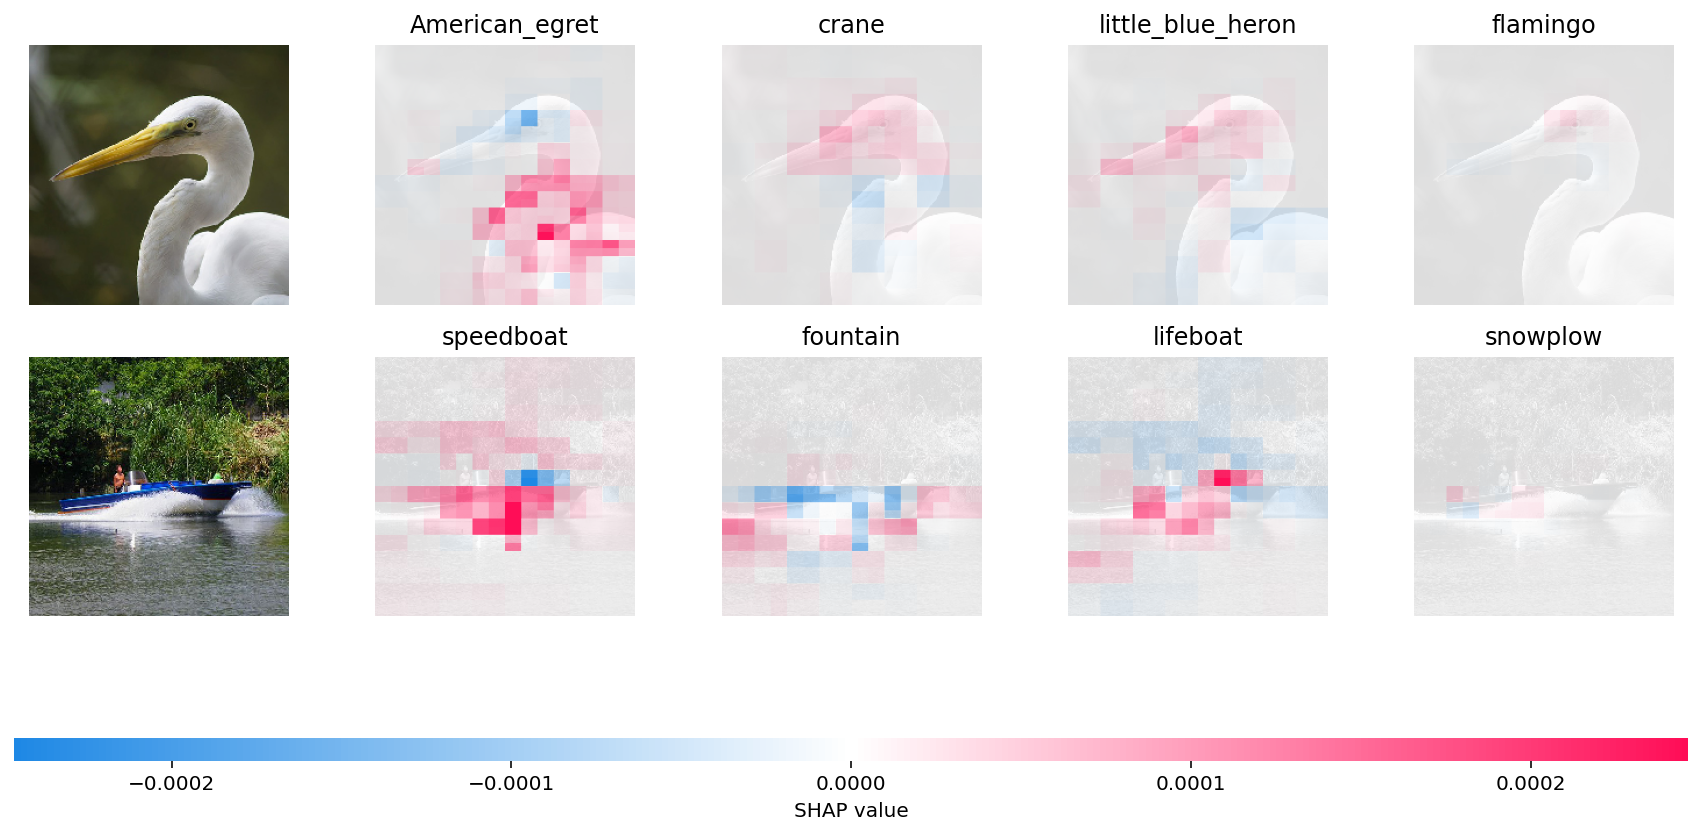
\includegraphics[width=.75\textwidth]{shap_image.png} \\

\scriptsize Source: \url{https://github.com/shap} (MIT License)
\caption{SHAP for image classification}
\label{fig:shapimage}
\end{figure}

\begin{figure}
\centering

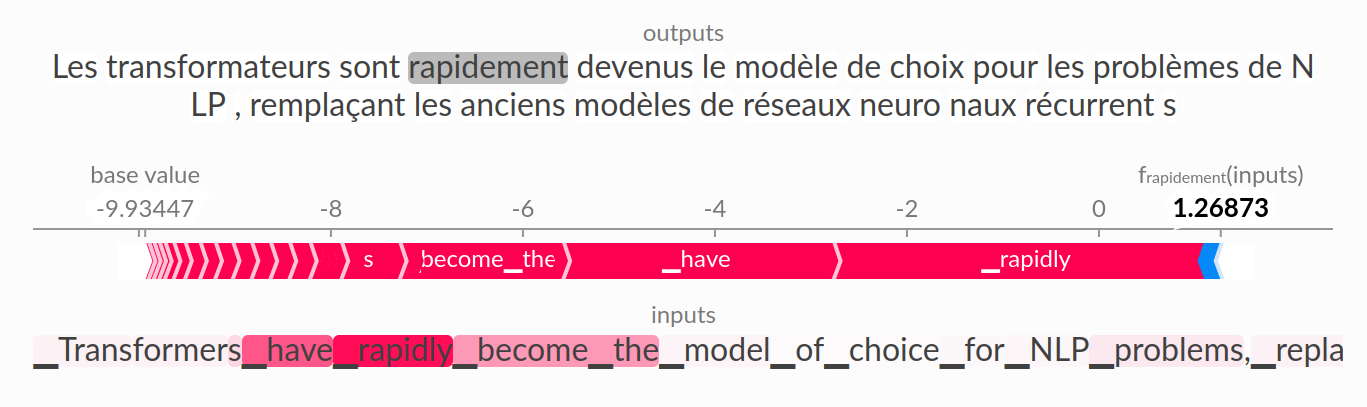
\includegraphics[width=.75\textwidth]{shap_text.png} \\

\scriptsize Source: \url{https://shap.readthedocs.io/en/latest/text_examples.html} (MIT License)
\caption{SHAP for text classification}
\label{fig:shaptext}
\end{figure}

\FloatBarrier
\section{Review Questions}
\paragraph*{Introduction to Interpretable Machine Learning}
\begin{enumerate}[nosep]
    \item List at least three reasons why interpretable machine learning is crucial in modern AI applications.
    \item What does it mean for a machine learning model to be ''interpretable''? Give examples of features that contribute to a model's interpretability.
    \item Discuss the trade-offs between model complexity and interpretability. Why might a more complex model be chosen over a simpler, more interpretable model?
    \item Provide examples of how interpretable machine learning can lead to innovations and improvements in AI systems.
    \item Why is the understanding of automated decisions particularly crucial in sectors like healthcare and finance?
    \item Discuss the relationship between interpretable machine learning and the ethical responsibilities of AI developers.
    \item Discuss the role of interpretable machine learning in ensuring safety, compliance, and reliability of AI systems.
    \item What is the importance of interpretable machine learning in detecting biases and ensuring fairness in model predictions?
    \item What factors should be considered when deciding between intrinsic and post-hoc interpretability methods in a given application?
    \item Compare and contrast local and global interpretation methods in terms of their applications and benefits.
    \item How do local and global interpretation methods complement each other in providing a comprehensive understanding of machine learning models?
    \item How do intrinsic and post-hoc methods affect the user's trust and acceptance of machine learning models?
\end{enumerate}
\paragraph*{Intrinsically Interpretable Models}
\begin{enumerate}[nosep,resume*]
    \item How do t-values contribute to understanding the relative importance of features in a linear regression model?
    \item What are decision trees, and how are they used in both regression and classification contexts in machine learning?
    \item Describe the structure of a typical decision tree and explain how decisions are represented within this structure.
    \item Explain why decision trees do not require normalization or scaling of data before analysis. What advantages does this present in terms of data preprocessing?
    \item Discuss the advantages of using decision trees in terms of algorithmic transparency. How does this feature contribute to their interpretability?
    \item Explain how decision trees handle non-linear relationships and the significance of this capability.
    \item Discuss how decision trees manage to capture interactions between variables without explicit programming for these interactions.
    \item What is overfitting in the context of decision trees, and why are decision trees particularly susceptible to it?
    \item Explain the process of making binary splits in decision trees, particularly how regions and leaf nodes are determined.
    \item Explain the various stopping criteria used in the construction of decision trees. Compare them in terms of their impact on tree complexity and performance.
    \item Discuss the implications of high variance in decision trees. What techniques can be used to mitigate this issue?
\end{enumerate}
\paragraph*{Global Model-Agnostic Methods}
\begin{enumerate}[nosep,resume*]
    \item What are Partial Dependence Plots (PDPs) and what do they show in a machine learning model?
    \item Explain the assumption of feature independence in PDPs and its implications.
    \item Describe a scenario where the assumption of feature independence in PDPs might lead to incorrect conclusions about feature importance.
    \item How can ICE plots help in identifying outlier effects or heterogeneity in data predictions?
    \item Describe how ALE plots differ from PDPs in their approach to understanding feature effects.
    \item Explain the computation process of ALE plots and how it differs fundamentally from PDPs in handling data within local windows.
    \item Discuss how ALE plots handle correlated features and why this is beneficial.
    \item What is Permutation Feature Importance and how is it calculated?
    \item Explain global surrogate models in interpretable machine learning.
    \item Discuss the potential risks or drawbacks of using global surrogate models as a tool for interpretability. What should practitioners be wary of?
    \item Compare and discuss the strengths and weaknesses of the global model-agnostic methods covered (PDP, ICE, ALE, PFI, and global surrogate models).
\end{enumerate}
\paragraph*{Local Interpretable Model-agnostic Explanations (LIME)}
\begin{enumerate}[nosep,resume*]
    \item What are local model-agnostic interpretative methods, and how do they differ from global interpretative methods?
    \item Outline the step-by-step process of generating a LIME explanation for a given data instance.
    \item Explain the purpose of transforming an instance into a binary vector in the LIME process. What does this achieve in terms of interpretability?
    \item Discuss the role of perturbing input data points in the LIME process. What is the purpose of creating ''synthetic'' samples?
    \item How does LIME ensure that the local surrogate model accurately reflects the behavior of the complex model in the vicinity of a specified data point?
    \item Identify potential pitfalls when applying LIME to a dataset with highly correlated features. How does this correlation affect the integrity of the explanations provided?
    \item Provide a critical analysis of how LIME handles cases where the local decision boundary is highly non-linear. What are the challenges and how might LIME overcome them?
    \item Reflect on the dependency of LIME's explanations on the kernel function. How can different kernels alter the interpretation of feature contributions?
\end{enumerate}
\paragraph*{Shapley Additive eXplanations (SHAP)}
\begin{enumerate}[nosep,resume*]
    \item Explain the concept of Shapley values in the context of cooperative game theory.
    \item Discuss the significance of treating each feature as a ''player'' in the context of SHAP. How does this perspective aid in understanding model predictions?
    \item Describe the four key theoretical properties of the Shapley value and explain how each contributes to fairness and accuracy in SHAP.
    \item Outline the steps to compute SHAP values for a machine learning model.
    \item Describe how SHAP values are visualized and interpret such a visualization.
    \item What insights can be gained from SHAP waterfall and beeswarm plots? 
    \item How can SHAP be integrated into the model development process to improve model design and feature engineering?
    \item Discuss the potential for SHAP to be used in regulatory compliance, specifically in industries like finance and healthcare. What advantages does SHAP offer in explaining model decisions to regulators?
\end{enumerate}
